\documentclass{article}

\usepackage{amssymb, amsmath, amsthm, tikz, verbatim, graphicx,lmodern,indentfirst,enumerate,color}

\usepackage[titletoc,page]{appendix}
\usepackage[margin=1.4in]{geometry}

\newtheorem{thm}{Theorem}[section]
\newtheorem{lem}[thm]{Lemma}
\newtheorem{prop}[thm]{Proposition}
\newtheorem{cor}[thm]{Corollary}
\newtheorem{con}[thm]{Conjecture}
\newtheorem{oprob}[thm]{Open Problem}
\newtheorem{prob}[thm]{Problem}

\theoremstyle{definition}
\newtheorem{example}[thm]{Example}

\theoremstyle{definition}
\newtheorem{question}[thm]{Question}

\theoremstyle{definition}
\newtheorem{defn}[thm]{Definition}

\theoremstyle{remark}
\newtheorem{rem}[thm]{Remark}

\numberwithin{equation}{section}

\newcommand*\circled[1]{\tikz[baseline=(char.base)]{
            \node[shape=circle,draw,inner sep=0pt,minimum size=5mm] (char) {#1};}}
\newcommand*\circleD[1]{\tikz[baseline=(char.base)]{
            \node[shape=circle,draw,inner sep=0pt,minimum size=7mm] (char) {#1};}}

\newcommand{\rootsG}[8]{\circled{#1}
            \begin{tabular}{cccccc}
             &&&#2&& \\
             #3&#4&#5&#6&#7&#8
             \end{tabular}}
\newcommand{\rootsE}[7]{\circled{#1}
            \begin{tabular}{ccccc}
             &&#2&& \\
             #3&#4&#5&#6&#7
             \end{tabular}}
\newcommand{\rootsC}[9]{\circleD{#1}
            \begin{tabular}{ccccccc}
             &&&&#2&& \\
             #3&#4&#5&#6&#7&#8&#9
             \end{tabular}}
\newcommand{\rootsD}[5]{\circled{#1}
            \begin{tabular}{ccc}
             &#2& \\
             #3&#4&#5
             \end{tabular}}
\makeatletter
\newcommand{\rmnum}[1]{\romannumeral #1}
\newcommand{\Rmnum}[1]{\expandafter\@slowromancap\romannumeral #1@}
\makeatother
\bibliographystyle{plain}
\begin{document}

%--------------------------------------------------------------
% title.tex (tesi.tex main file)
%--------------------------------------------------------------
\begin{titlepage}
	\begin{center}
		\large
		\hfill
		\vfill
		\begingroup
			\spacedallcaps{\myUni}\\
			\myFaculty \\
			\myDegree \\ 
			\vspace{0.5cm}
			\includegraphics[scale=.065]{unifi.pdf}\\
			\vspace{0.5cm}
			Tesi di Laurea
		\endgroup
		\vfill
		\begingroup
			\color{Maroon}\spacedallcaps{\myTitle}\\
			\spacedlowsmallcaps{\mySubtitle}\\
			\bigskip
		\endgroup
		\spacedlowsmallcaps{\myName}
		\vfill
		Relatore: \textit{\myProf}\\
		Correlatore: \textit{\mySupervisor}
		\vfill
		\myTime
		\vfill
	\end{center}
\end{titlepage}
%--------------------------------------------------------------
% back titlepage
%--------------------------------------------------------------
\newpage
	\thispagestyle{empty}
	\hfill
	\vfill
	\noindent\myName: \textit{\myTitle: \mySubtitle,} \myDegree, \textcopyright\ \myTime
%--------------------------------------------------------------
% back titlepage end
%--------------------------------------------------------------

\section{Introduction}
\label{sec:Introduction}


The goal in top-$\size$ recommendation is to recommend to each
consumer a small set of $\size$ items from a large collection of
items~\cite{cremonesi2010performance}.  For example, Netflix may want
to recommend $\size$ appealing movies to each consumer.  Collaborative
Filtering (CF)~\cite{herlocker2002empirical,lee2012comparative} is a
common top-$\size$ recommendation method.  CF infers user interests by
analyzing partially observed user-item interaction data, such as user
ratings on movies or historical purchase
logs~\cite{kanagal2012supercharging}. The main assumption in CF is that
users with similar interaction patterns have similar interests.


Standard CF methods for top-$\size$ recommendation focus on making  suggestions  that accurately reflect the user's preference history. However, as  observed in previous work,  CF recommendations are generally biased toward  popular items, leading to a rich get richer effect~\cite{vargas2014improving,steck2011item}.  The major reasons for this are \textit{popularity bias} and \textit{sparsity} of CF interaction data (detailed in Section~\ref{sec:related-work}). In a nutshell, to maintain  accuracy, recommendations are generated from the dense regions of the data,  where the popular items lie.  

However,  accurately suggesting popular items, may not be satisfactory for the consumers. For example, in Netflix, an accuracy-focused movie recommender may recommend ``Star Wars: The Force Awakens'' to users who have seen ``Star Wars: Rogue One''.  But, those users are probably already aware of ``The Force Awakens''. Considering additional factors, such as novelty of recommendations,  can lead to more effective suggestions~\cite{cremonesi2010performance,Castells2015,zhang2008avoiding,ziegler2005improving,zhang2012auralist}. 
%Second, accuracy-focused models typically achieve a   overall item-space coverage across their recommendations,  whereas high item-space coverage helps providers of the items increase revenue
%, users satisfaction since they are  likely already aware of or can find these items on their own.  

Focusing on popular items also adversely affects the satisfaction of  the providers of the items. This is because  accuracy-focused models typically achieve a  low overall item space coverage across their recommendations, whereas   high item space coverage helps providers of the items increase their revenue~\cite{vargas2014improving,Castells2015,adomavicius2011maximizing,anderson2006thelongtail, yin2012challenging,adomavicius2012improving}.
%accuracy-focused models typically achieve a

In contrast to the relatively small number of popular items, there are copious  {\it long-tail\/} items that have fewer observations (e.g., ratings) available. More precisely,  using the Pareto  principle (i.e.,~the $80/20$ rule),  long-tail items can be defined as items that generate the lower $20\%$ of observations~\cite{yin2012challenging}. Experimentally we found that these items correspond to almost $85\%$ of the items in several datasets (Sections~\ref{sec:Notation} and \ref{sec:Experiments}). %Table~\ref{tab:DatasetStatsticsSmall})


As previously shown, one way to improve the novelty of top-$\size$ sets is to recommend interesting long-tail items~\cite{cremonesi2010performance,ge2010beyond}.  The intuition  is that since they have fewer observations available,  they are more likely to be unseen~\cite{Kaminskas:2016:DSN:3028254.2926720}.  
 %For example, in online commerce,  newly added items are long-tail items that are yet to be discovered.  
Moreover, long-tail item promotion also results in higher overall coverage of the item space%, which increases profits for providers of the items
~\cite{vargas2014improving,Castells2015,zhang2008avoiding,zhang2012auralist,adomavicius2011maximizing,anderson2006thelongtail,yin2012challenging,jambor2010optimizing}. Because long-tail promotion reduces accuracy~\cite{steck2011item}, there are trade-offs to be explored.


%original submitted to ICDE
%This work studies three aspects of top-$\size$ recommendation: accuracy, novelty, and item-space coverage, and examines their trade-offs. In most previous work, predictions of a base recommendation system are re-ranked to handle their trade-offs~\cite{adomavicius2012improving,jambor2010optimizing,zhang2013personalize,wang2009portfolio}. Due to performance considerations, however, these techniques are not customized per user. For example,  parameters that balance the trade-off between novelty and accuracy are cross-validated at a global level.  This can be detrimental since users have varying preferences for  objectives such as long-tail novelty. We explore how to  automatically infer  user  preference for long-tail novelty, and how to leverage  it to correct  the popularity bias in standard recommender models. Our work does not rely on any additional contextual data, although such data, if available, can help promote newly-added long-tail items~\cite{agarwal2009regression,Saveski:2014:ICR:2645710.2645751}.

This work studies three aspects of top-$\size$ recommendation: accuracy, novelty, and item space coverage, and examines their trade-offs. In most previous work, predictions of a base recommendation algorithm are \textit{re-ranked} to handle these trade-offs~\cite{adomavicius2012improving,jambor2010optimizing,zhang2013personalize,wang2009portfolio}. The re-ranking models are computationally efficient but suffer from two drawbacks. First, due to performance considerations,  parameters that balance the trade-off between novelty and accuracy  are not customized per user. Instead they are cross-validated at a global level.  This can be detrimental since users have varying preferences for  objectives such as long-tail novelty. Second,  the re-ranking methods are often limited to a specific base recommender  that may be sensitive to dataset density. 
As a result, the datasets are pruned and the problem is studied in dense settings~\cite{adomavicius2012improving,ho2014likes}; but real world  scenarios are often sparse~\cite{kanagal2012supercharging,liu2017experimental}.   
% Because  dataset density can impact the performance of most base recommenders (like R-SVD), which in turn affects the performance of the re-ranking model, 

\iffalse
We address these limitations by directly inferring  user  preference for long-tail novelty  from interaction data.  This  allows us to customize the re-ranking  per user, and design a \textit{generic} framework, which resolves the second problem. In particular, since the long-tail novelty preferences are estimated independently of any base  recommender model, we can  plug-in an appropriate base recommender w.r.t. the dataset sparsity.% including ones that are more suitable for sparse settings.  

Modelling  user  preference for  long-tail novelty using only item popularity statistics, e.g., the average popularity of rated items as in~\cite{jugovac2017efficient}, disregards additional information like whether the user found the item interesting and the long-tail preferences of other users  of the items. \iffalse To incorporate them, we introduce the notion of  \emph{item long-tail importance}. Both  user long-tail preferences and item long-tail importance are dependent:  a user has high preference for discovering long-tail items if she is interested in important long-tail items, and an item that is associated with many of these kinds of users is likely to be more important.  We propose a joint optimization framework to directly learn,  from interaction data, both the users' long-tail preferences and the  items' long-tail importance. \fi
We propose an optimization approach that  incorporates  this information and  directly learns,  from interaction data, the users' long-tail novelty preferences.

Next, we use these learned preferences  to design a  top-$\size$ recommendation framework thats is generic, and provides customized balance between accuracy, novelty, and coverage. We refer to it as framework as GANC.  Using GANC, we design a novel algorithm, {\it Ordered Sampling-based Locally Greedy (OSLG)\/}, that relies on the learned long-tail novelty preferences  to scalably correct for popularity bias. Our work does not rely on any additional contextual data, although such data, if available, can help promote newly-added long-tail items~\cite{agarwal2009regression,Saveski:2014:ICR:2645710.2645751}. In summary:
\fi

We address the first limitation by directly inferring  user  preference for long-tail novelty  from interaction data.   Estimating these  preferences  using only item popularity statistics, e.g., the average popularity of rated items as in~\cite{jugovac2017efficient}, disregards additional information, like whether the user found the item interesting or the long-tail preferences of other users  of the items. We propose an approach that  incorporates  this information and  learns the users' long-tail novelty preferences from interaction data.

This approach allows us to customize the re-ranking  per user, and  design a \textit{generic} re-ranking framework, which resolves the second limitation of prior work. In particular, since the long-tail novelty preferences are estimated independently of any base recommender, we can  plug-in an appropriate one w.r.t. different factors, such as the dataset sparsity.

Our top-$\size$ recommendation framework, \textbf{GANC}, is \textbf{G}eneric, and provides customized balance between \textbf{A}ccuracy, \textbf{N}ovelty, and \textbf{C}overage. % Moreover, based on the learned long-tail novelty preferences, we also design a novel algorithm, {\it Ordered Sampling-based Locally Greedy (OSLG)\/}, that relies on the learned long-tail novelty preferences  to scalably correct for popularity bias. 
Our work does not rely on any additional contextual data, although such data, if available, can help promote newly-added long-tail items~\cite{agarwal2009regression,Saveski:2014:ICR:2645710.2645751}. In summary:

%Consider  the following toy example:
\vspace{-0.2cm}
\begin{table}[htb]
\centering
\scriptsize
%\small
\begin{tabular}{ccccccc} 
%\toprule
%&\multirow{2}{*}{}&\multicolumn{7}{c}{Ratings}\\
& & \cellcolor{blue!35}$w_1$ &\cellcolor{blue!18} $w_2$ & $\dots$ &\cellcolor{blue!8} $w_{89}$  &\cellcolor{blue!8} $w_{99}$   
\\
&   &$i_1$&$i_2$&$\dots$&$i_{89}$&$i_{90}$\\ 
\cmidrule(r){3-7} 	 
%\midrule
\cellcolor{red!35}$\theta_1$  &$u_1 $   &5 &   & $\dots$ &  &   \\
\cellcolor{red!28}$\theta_2$  &$u_2$     &5 &    & $\dots$ &  &  \\
 $\theta_3=?$  &$\bf u_3$  &5 &  &   $\dots$ &  &  \\
\cellcolor{red!10}$\theta_4$ & $u_4$  &  &5   & $\dots$ & &\\ 
\cellcolor{red!10}$\theta_5$ & $u_5$  &  & 5  & $\dots$ & &\\ 
$\theta_6=?$  & $\bf u_6$ & &5  &      $\dots$& &  \\ 
 & & $\hdots$  &$\hdots$   &$\hdots$   &$\hdots$   &$\hdots$  \\
%\midrule 
\cmidrule(r){3-7} 	 
\multicolumn{2}{c}{item pop.}  & 3  & 3  & $\dots$ &50&60\\  
%\bottomrule
%$ f_i$    &3  &3  &1  &3  &1  &2  \\  \hline
\end{tabular}
%#.
\caption{Simplified user-item interaction data. The user long-tail novelty preference ($\theta_u$), item long-tail importance weight ($w_i$) are highlighted. Darker colors indicate larger values. } \label{tab:example}
\end{table} 
\vspace{-0.2cm}
\begin{example}  
In Table~\ref{tab:example}, we are interested in estimating $\theta_3$ and $\theta_6$,  the long-tail preference of users $u_3$ and $u_6$ who have each rated a single movie. Additional ratings for other users  are not included here.  Considering only rating information, we observe $i_1$ and $i_2$ are  equally popular $|\mathcal{U}_{i_1}^{\trainset}| = |\mathcal{U}_{i_2}^{\trainset}|=3$, and $r_{31}=5$ and $r_{62}=5$. Using Eq.~\ref{eq:tfidf-risk}  we have $\theta_3 = \theta_6$. However, if we were given the long-tail preferences of the each item's user set, specifically that $u_1$ and $u_2$ have high long-tail preference (darker red), while $u_4$ and $u_5$ have lower long-tail preference (lighter red), we could conclude $i_1$ is a more important long-tail item compared to $i_2$ (indicated by a darker blue shade for $w_1$), and we expect  $\theta_3 \geq \theta_6$.

% On the other hand, if we knew that $u_4$ and $u_5$ have lower long-tail preference, we could conclude $i_2$ is a  less significant long-tail item. Therefore, However, if we  consider the long-tail preferences of other users, we may reason differently.    We need another variable $w_i$ which captures this information. 
%we would conclude that $u_3$ has higher long-tail preference compared to $u_6$, since the users $i_1$ is a more prominent long-tail item. 

% Relying only  on item popularity information, we would  conclude   $u_3$ and $u_6$ have equal long-tail preference, since $i_1$ and $i_2$ are  equally popular. However, considering  the second column,  long-tail preference of users,  long-tail importance for each item,  which captures the long-tail preference of its users. Since  that  both users of $i_1$ have high long-tail preference while  the users of $i_2$ have lower preference,  we may conclude $i_1$ is a more important long-tail item compared to $i_2$. Therefore, $u_3$'s long-tail preference should be at least as large as $u_6$'s preference. Specifically, consider two  items $i_1$ and $i_2$, with the following rating data: $i_1=\{u_1:5, u_2:5, u_3:5 \}$, $i_2=\{u_4:5, u_5:5, u_6:5\}$.  

%Table~\ref{tab:example} shows  simplified rating data. We want an estimate of the long-tail preference of $u_3$ and $u_6$, who have each  rated a single movie.  Relying only  on movie popularity information, we would  conclude   $u_3$ and $u_6$ have similar long-tail preference, since $m_1$ and $m_2$ are  equally popular. However, considering the long-tail preferences of other users of those movies, we may reason differently: since $u_1$ and $u_2$ have high long-tail preference, and $u_4$ and $u_5$ have low long-tail preference, $m_1$ is a more prominent long-tail item compared to $m_2$. Therefore, it is likely that $u_3$ has higher long-tail preference compared to $u_6$.considering the long-tail preferences of other users of those movies, we may reason differently.  For example, 
\label{ex:running}
\end{example}



%------------------------------

\iffalse
\begin{example}
Table~\ref{tab:example} shows rating data for a simplified system. %Note the user-item interaction matrix is sparse.
For this example, we define popular movies as those that have received  three or more ratings; $\{m_1, m_2, m_4\}$ are popular and  $\{m_3, m_5, m_6\}$ are niche movies. We observe $u_1$ and $u_3$  have rated relatively popular movies (risk-averse) while $u_2$ and $u_4$ have rated niche movies (risk-loving). 
\label{ex:running}
\end{example}

\begin{table}[htb]
\centering
\scriptsize
\begin{tabular}{ccccccc} 
\toprule
			&$m_1$ &$m_2$   &$m_3$    &$m_4$   &$m_5$ &$m_6$  \\ \hline 
$u_1 $ &5  &4  & - &-  &-  &-   \\
$u_2$  &-  &-  &-  &-  &5  &5   \\
$u_3$  &-  &4  &-  &5  &-  &-   \\
$u_4$  &-  &-  &3  &-  &-  &4   \\ 
$u_5$  &5  &-  &-  &3  &-  &-   \\ 
$u_6$  &4  &2  &-  &4  &-  &-   \\ 
\bottomrule
%$ f_i$    &3  &3  &1  &3  &1  &2  \\  \hline
\end{tabular}
\caption{User-Movie rating data} \label{tab:example}
\end{table}

It is essential to consider consumer characteristics in designing recommender systems so that they promote long-tail items to the right group of users and spread demand evenly between hit and niche items.  

\fi





%------------------------------
\iffalse
\begin{table}[htb]
\centering
\scriptsize
\begin{tabular}{ccccccc} 
\toprule
			&$m_1$ &$m_2$   &$m_3$    &$m_4$   &$m_5$ &$m_6$  \\ \hline 
$u_1 $ &\textbf{5}  & \textbf{4}  &\textcolor{gray}{ 1.2} &-  &-  &-   \\
$u_2$  &-  &-  &-  &-  & \textbf{5}  &\textbf{5}   \\
$u_3$  &-  &\textbf{4}  &-  &\textbf{5}  &-  &-   \\
$u_4$  &-  &-  &\textbf{3}  &-  &-  &\textbf{4}   \\ 
$u_5$  &\textbf{5}  &-  &-  &\textbf{3}  &-  &-   \\ 
$u_6$  &\textbf{4}  &\textbf{2}  &-  &\textbf{4}  &-  &-   \\ 
\bottomrule
%$ f_i$    &3  &3  &1  &3  &1  &2  \\  \hline
\end{tabular}
\caption{User-Movie rating data} \label{tab:example}
\end{table}
% $\mathcal{P}^1= \{ \mathcal{P}_1^1 \{i_1,i_2,i_3\}, \mathcal{P}_2^1:\{i_2,i_3,i_5\}  \}$
 %$\mathcal{P}^2= \{ \mathcal{P}_1^2: \{i_1,i_2,i_3\}, \mathcal{P}_2^2:\{i_2,i_5,i_6\}  \}$
 %$\mathcal{P}^3= \{ \mathcal{P}_1^3: \{i_7,i_8,i_9\}, \mathcal{P}_2^3:\{i_{10},i_{11},i_{12}\}  \}$
\begin{table}[htb]
\centering
\tiny
\begin{tabular}{ccc} 
\toprule
		&$u_1$&$u_2$  \\ \hline 
$\mathcal{P}^1 $ & $\{i_1,i_2,i_3\}$ & $\{i_2,i_3,i_5\} $ \\
$\mathcal{P}^2$ & $\{i_1,i_2,i_3\}$ & $\{i_2,i_5,i_6\} $ \\
$\mathcal{P}^3$ & $\{i_7,i_8,i_9\}$ & $\{i_{10},i_{11},i_{12} \}$ \\
\bottomrule
%$ f_i$    &3  &3  &1  &3  &1  &2  \\  \hline
\end{tabular}
\caption{Top-$\size$ allocations to users.} \label{tab:paretoExamples}
\end{table}
\fi


\iffalse
When considering long-tail items, it is important to consider consumers' willingness  to explore niche or unpopular items and their propensity towards similar items. In particular, they can be characterized by their  {\it risk degree\/} and {\it focusing degree\/}, respectively.  We compute these estimates  based on historical rating information. The following example further describes these notions in the context of movie rating data. 

\begin{example}  
Table~\ref{tab:example} shows rating data for a simplified system with $6$ users, $6$ movies, and $3$ genres. $m_i^{j}$ implies that movie $m_i$ belongs to genre $j$. Note the user-item interaction matrix is sparse. 
  For this setting, we define popular movies as those that have received  three or more ratings; $\{m_1, m_2, m_4\}$ are popular and  $\{m_3, m_5, m_6\}$ are niche movies. We now profile the users according to their risk and focusing degree. E.g., $u_1$ has rated relatively popular movies belonging to the same genre (risk-averse, high focusing degree); $u_2$ has rated niches movies in the same genre (risk-loving, high focusing degree); $u_3$ has rated popular movies in two different genres (risk-averse, low focusing degree), and $u_4$ has rated niches movies in two different genres (risk-loving, low focusing degree). 
\label{ex:running}
\end{example}
\begin{table}[htb]
\centering
\tiny
\begin{tabular}{ccccccc} 
\toprule
			&$m_1^{1}$ &$m_2^{1}$   &$m_3^{2}$    &$m_4^{3}$   &$m_5^{3}$ &$m_6^{3}$  \\ \hline 
$u_1 $ &5  &4  &-  &-  &-  &-   \\
$u_2$  &-  &-  &-  &-  &5  &5   \\
$u_3$  &-  &4  &-  &5  &-  &-   \\
$u_4$  &-  &-  &3  &-  &-  &4   \\ 
$u_5$  &5  &-  &-  &3  &-  &-   \\ 
$u_6$  &4  &2  &-  &4  &-  &-   \\ 
\bottomrule
%$ f_i$    &3  &3  &1  &3  &1  &2  \\  \hline
\end{tabular}
\caption{User-Movie rating data} \label{tab:example}
\end{table}
It is essential to consider these consumer characteristics in designing recommender systems so that they promote long-tail items to the right group of users and spread demand evenly between the hit and niche items.  
\fi
\iffalse
\begin{center}
\begin{figure*}[tp]
%\scalebox{0.5}{%
\resizebox{1\textwidth}{!}{%
%\small%\addtolength{\tabcolsep}{5pt}% below sums to 8
\begin{tabularx}{1.5\textwidth}{>{\hsize=2.5\hsize}X>{\hsize=2.5\hsize}X>{\hsize=0.5\hsize}X>{\hsize=0.5\hsize}X>{\hsize=0.5\hsize}X>{\hsize=0.5\hsize}X>{\hsize=0.5\hsize}X>{\hsize=0.5\hsize}X}
    \multirow{12}{*}{\includegraphics[scale=0.3]{codeForExample/popularity-movie.png}} & \multirow{12}{*}{\includegraphics[scale=0.3]{codeForExample/scatterplot.png}} & & & & & & \\
%   & &               &       &       &       &       &       \\
    & &\multicolumn{1}{l|}{}               &$m_1^{g1}$   	&$m_2^{g1}$    	&$m_3^{g2}$    &$m_4^{g2}$      &$m_5^{g3}$    \\ \cline{3-8}%\hline
    & &\multicolumn{1}{l|}{u1}          &5  &5  &-  &-   &-  \\
    & &\multicolumn{1}{l|}{u2}    		&-  &-  &4  &4  &5  \\
    & &\multicolumn{1}{l|}{u3}   			&1  &2  &1  &-  &-   \\
    & &\multicolumn{1}{l|}{u4}     		&1  &-  &-  &-  &-  \\
    & &               &       &       &       &       &       \\
    & &               &       &       &       &       &       \\
    & &               &       &       &       &       &       \\
    & &               &       &       &       &       &	\\
    \\
\end{tabularx}}
\caption{User-Movie interaction data a) Popularity-Movie histogram b)Movie genres/clusters c) User-Movie rating data} \label{fig:example}
\end{figure*}
\end{center}
\fi



%We propose a novel approach that allows us to  promote long-tail items in a targeted manner, thereby improving the novelty of top-$\size$ sets, the overall item-space coverage across recommendations, while maintaining reasonable levels of accuracy.

%Next, we integrate these learned preferences  in a generic  top-$\size$ recommendation framework to provide customized balance between accuracy and coverage.

%sequentially make recommendations, while adjusting its parameters with regard to the set of top-$\size$ recommendations made so far. However, since  sequential parameter updates  cause  scalability issues, we propose a sampling based algorithm. This variant of our framework, called {\it Ordered Sampling-based Locally Greedy (OSLG)\/},  allows us to  correct for the popularity bias in recommendations with regard to individual user long-tail preferences. 

%ICDE submission
%Our framework differs with  prior work in the following aspects:  unlike~\cite{adomavicius2011maximizing,adomavicius2012improving,zhang2013personalize,ho2014likes},  the long-tail preference personalization in our framework is learned rather than optimized using cross-validation or parameter tuning. In other words, our personalization method is independent of the underlying base  recommendation models.  Moreover, our framework is  generic. This enables us to  plug-in several base recommenders, and evaluate their  effectiveness without requiring  extensive tuning for the accuracy and coverage trade-off. 


%\vspace{-2.8pt}
\begin{itemize}

\item  We examine various measures for estimating user long-tail novelty preference in Section~\ref{sec:lt-pref} and formulate an optimization problem  to directly learn users' preferences for long-tail  items from interaction data in Section~\ref{sec:learning-lt-pref}. %In addition, we introduce several heuristics for measuring the user preference for less common items from historical rating data.% 

\item  We integrate the user preference estimates into GANC %, a generic re-ranking framework that provides customized balance between accuracy, novelty, and coverage 
(Section~\ref{sec:RiskbasedReranking}), and  introduce {\it Ordered Sampling-based Locally Greedy (OSLG)\/}, a scalable algorithm that relies  on user long-tail preferences to correct the popularity bias (Section~\ref{sec:optimizationAlgorithm}).
%We introduce OSLG, a scalable algorithm that relies  on user long-tail preferences to  maximize item space coverage \textcolor{red}{while maintaining acceptable levels of accuracy} (Section~\ref{sec:optimizationAlgorithm}).

\item   We conduct an extensive empirical study and evaluate performance from  accuracy, novelty, and coverage perspectives (Section~\ref{sec:Experiments}).  We use five  datasets with varying density and difficulty levels. %:  Netflix, MovieTweetings, and MovieLens (100K, 1M, 10M). 
  In contrast to most related work,  our evaluation considers realistic settings that include a large number of infrequent  items and users. %This enables us to study the impact of  data density on the performance trade-offs of several  state of the art top-$\size$ recommendation algorithms. %   %,  and use the all-items ranking protocol~\cite{steck2013evaluation,vargas2014improving}, where performance is measured using all items with train data. to evaluate the performance of several  state of the art top-$\size$ recommendation algorithms 
 
\item Our empirical results confirm that the performance of re-ranking models is impacted by the underlying   base recommender and the dataset density. Our generic approach enables us to easily incorporate a suitable base recommender to devise an effective solution for both dense and sparse settings. In dense settings, we use the same base recommender as existing re-ranking approaches, and we outperform them in accuracy and coverage metrics. For sparse settings, we plug-in a more suitable base recommender, and devise an effective solution that is competitive with existing top-$\size$ recommendation methods in accuracy and novelty. 

%Directly estimating the long-tail novelty preferences allows us to customize re-ranking per user, and  devise a generic framework.   
 
\end{itemize}

Section~\ref{sec:related-work} describes related work. Section~\ref{sec:conclusion} concludes.

\section{The causal structure of doubly warped spacetimes}
\label{sec:chronologicalrelation}
%By a {\em \multiwarped spacetime} we understand a lorentzian manifold $(V,g)$ where
%\begin{equation}
%  \label{eq:1}
%  V:= \R \times M_{1} \times M_{2}\quad\hbox{and}\quad
%g=-dt^{2}+\alpha_{1}g_{1}+\alpha_{2}g_{2},
%\end{equation}
%being $(M_{i},g_{i})$ a Riemannian manifold for $i=1,2$.
%
%\smallskip

In this section we are going to characterize the chronological and causal relations in doubly warped spacetimes. First, recall that a {\em \multiwarped spacetime} is a multiwarped spacetime $(V,g)$ as in (\ref{eqqq}) with two fibers ($n=2$), that is,

\begin{equation}
  \label{eq:1-aux}
  V:= (a,b)\times M_{1} \times M_{2}\quad\hbox{and}\quad
g=-dt^{2}+\alpha_{1}g_{1}+\alpha_{2}g_{2}.
\end{equation}
%where $\alpha_i:\R\rightarrow (0,\infty)$ are positive smooth functions and $(M_{i},g_{i})$ are Riemannian manifolds for $i=1,2$.
%\begin{rem}\label{rem:infinito}
%Since the structures studied in this paper are invariant by conformal transformations, our analysis implicitly covers the case where the temporal interval $(a,b)$ is a proper subset of $\R$. In fact, otherwise, multiply the metric by an appropriate positive function in order to obtain another doubly warped spacetime in the same conformal class with $(a,b)=\R$.
%\end{rem}




%\begin{rem}\label{rem:infinito}
%  As we are going to be interested in causal structures, there is no loss of generality if we assume that $(a,b)\equiv \R$. In fact, given a metric as in \eqref{eq:1-aux}, let us consider $\beta:(a,b)\rightarrow (0,\infty)$ a function satisfying that:
%  \[
%\int_{c}^b \frac{1}{\sqrt{\beta(t)}}dt=\infty=\int_{a}^c\frac{1}{\sqrt{\beta(t)}}dt
%    \]
%    for some $c\in (a,b)$. Then,
%    \[
%      \begin{array}{rl}
%        {\mathfrak g}=& -dt^{2}+\alpha_{1}g_{1}+\alpha_{2}g_{2}\\ =& \beta \left(-\left(\frac{dt}{\sqrt{\beta}}\right)^2+ \frac{\alpha_1}{\beta}g_1+\frac{\alpha_2}{\beta}g_2\right)\\ = & \beta \left(-ds^2+\tilde{\alpha}_1g_1+\tilde{\alpha}_2g_2   \right) \\ =&\beta\, g,
%      \end{array}
%      \]
%      where $s\in \R$ as, from definition, $ds=dt/\sqrt{\beta}$. Moreover,
%
%      \[
%\int_{0}^{\infty} \frac{1}{\sqrt{\tilde{\alpha}_i(s)}}ds=\int_{c}^{a} \frac{1}{\sqrt{\alpha_i(t)}}dt, \qquad \int_{0}^{-\infty} \frac{1}{\sqrt{\tilde{\alpha}_i(s)}}ds=\int_{c}^{b} \frac{1}{\sqrt{\alpha_i(t)}}dt, \quad\hbox{ for $i=1,2$}.
%        \]
%        In conclusion, the metric $\mathfrak{g}$ is conformal to $g$, which is also a {\multiwarped} model where the time component belongs to the entire $\R$ and with warping functions preserving some integral condition. Therefore, unless stated otherwise (essentially, on the main results), we will always work considering {\multiwarped} models as follow:
%
%        \begin{equation}
%  \label{eq:1}
%  V:= \R \times M_{1} \times M_{2}\quad\hbox{and}\quad
%g=-dt^{2}+\alpha_{1}g_{1}+\alpha_{2}g_{2},
%\end{equation}
%
%\end{rem}
%}


Take $(t^e,x^e)\in V$ and $x^o\in M:=M_1\times M_2$. Denote by $C(x^o,x^e)$ the set of smooth curves in $M$ connecting $x^o$ with $x^e$. Given $c=(c_1,c_2)\in C(x^o,x^e)$, consider the unique future-directed lightlike curve $\rho:[s^o,s^e]\rightarrow V$ with $\rho(s)=(\tau_{c,t^e}(s),c(s))$ and $\tau_{c,t^e}(s^e)=t^e$. From the metric expression in (\ref{eq:1-aux}), the component $\tau_{c,t^e}(s)$ is determined by the Cauchy problem
\[
-\dot{\tau}_{c,t^e}^2+\alpha_1(\tau_{c,t^e})g_{1}(\dot{c}_1,\dot{c}_1)+\alpha_2(\tau_{c,t^e})g_{2}(\dot{c}_2,\dot{c}_2)=0,\qquad
    \tau_{c,t^e}(s^e)=t^e.
  \]
Consider the functional
\[\J_{x^o,(t^e,x^e)}: C(x^o,x^e) \rightarrow (a,b), \quad c \mapsto \tau_{c,t^e}(s^o).\]
A direct computation shows that $(t^o,x^o)\ll (t^e,x^e)$ if, and only if, there exists $c\in C(x^o,x^e)$ such that $t_o<\J_{x^o,(t^e,x^e)}(c)$. This property suggests the following definition for the {\em departure time function}:
\[
T:M\times \left((a,b)\times M\right)\rightarrow (a,b),\qquad T(x^{o},(t^{e},x^{e})):= {Sup}_{C}\J_{x^o,(t^e,x^e)}
\]
(compare with \cite[Section 2.9]{Perlick2004} and \cite[Section 4]{FS2}). By construction, this function characterizes the chronological relation in $(V,g)$, as follows:
\begin{equation}\label{e0}
(t^{o},x^{o}) \ll (t^{e},x^{e}) \;\; \Longleftrightarrow \;\;
t^{o}<T(x^{o},(t^{e},x^{e})).
\end{equation}
In particular, the chronological past of a given point $(t^e,x^e)$ is given by
\[
I^-\left((t^e,x^e) \right):=\{(t,x)\in (a,b)\times M: t<T(x,(t^e,x^e)) \}.
  \]
Given a future-directed timelike curve $\gamma(t)=(t,c(t))$, $t\in [\omega,\Omega)$, and a point $x\in M$, the transitivity of the chronological relaction $\ll$ ensures that the function $T(x,\gamma(t))$ is increasing on $t$. Hence, the chronological past of $\gamma$ can be written as
  \[
I^-(\gamma)=\{(s,x)\in (a,b)\times M: s<b_c(x):=lim_{t\rightarrow b}T(x,\gamma(t))\}.
    \]
%    \begin{rem}
%      The choice of $b_c$ to denote such a limit came motivated from the studies of the causal boundary for standard static  spacetimes, that can be considered as... In fact, as it can be deduced from CITA REQUERIDA, $T(x,(t^*,y))=t^*-d(x,y)$, and so, when...\footnote{Simplemente concretar lo anterior al caso estático estandar, a modo de ejemplo.}.
%    \end{rem}

Next, let us characterize the departure time function, and so, the chronological relations (recall (\ref{e0})), in terms of some integral conditions involving the warping functions $\alpha_i$ and the Riemannian distances $d_i$ associated to the fibers $(M_i,g_i)$, $i=1,2$.
To this aim, let us consider a future-directed causal curve $\gamma:  I \rightarrow V$,
$\gamma(s)=(t(s),c_{1}(s),c_{2}(s))$. From the metric expression in \eqref{eq:1-aux}:
\[
\frac{dt}{ds}(s)=\sqrt{-D+\frac{\mu_{1}}{\alpha_{1}\circ
t}+\frac{\mu_{2}}{\alpha_{2}\circ t}}(s),
\]
where $D:=g(d\gamma/ds,d\gamma/ds)\leq 0$ and
$\mu_{i}:=(\alpha_{i}\circ t)^2 g_{i}(dc_{i}/ds,dc_{i}/ds)$,
$i=1,2$. From the Inverse Function Theorem, previous formula translates into
\[
\frac{ds}{dt}(t)=\left(-(D\circ s)+\frac{\mu_{1}\circ s}{\alpha
_{1}}+\frac{\mu_{2}\circ s}{\alpha _{2}}\right)^{-1/2}.
\]
Therefore, if we denote $t^{o}=t(s^{o})$, $t^{e}=t(s^{e})$, we
deduce
\begin{equation}\label{eq:3}
\begin{array}{c}
\hbox{length}\left(c_{i}\mid_{[s^{o},s^{e}]}\right)=\int_{s^{o}}^{s^{e}}\sqrt{g_{i}(\dot
c_{i}, \dot c_{i})} ds=\int_{t^o}^{t^e}\sqrt{g_{i}(\dot c_{i}, \dot
c_{i})} \frac{ds}{dt} dt \qquad\qquad\qquad\quad \\
\;\quad\qquad\qquad\qquad =\int_{t^o}^{t^e}\frac{\sqrt{\mu_{i}\circ
s}}{\alpha_i(t)}\left(-(D\circ s)+\frac{\mu_{1}\circ
s}{\alpha_{1}(t)}+\frac{\mu_{2}\circ s}{\alpha_{2}(t)}\right)^{-1/2}dt
\qquad\hbox{for}\;\; i=1,2.
\end{array}
\end{equation}
In the particular case of being $\gamma$ a lightlike geodesic we have: (i) $D=0$ (lightlike character of $\gamma)$, (ii) $\mu_i\circ s$ are constants and (iii) $c_i$ are (pre-)geodesics on the corresponding Riemannian manifold $(M_i,g_i)$ (geodesic character of $\gamma$). So, from (\ref{eq:3}), one deduces (see \cite[Theorem 2]{FS} for details):
\begin{prop}\label{thm:characluzgeodesics}
  Let $(V,g)$ be a {\multiwarped} spacetime as in (\ref{eq:1-aux}) with (weakly) convex fibers (i.e., satisfying that any pair of points can be joined by some minimizing geodesic). Consider two distinct points $(t^o,x_1^o,x_2^o),(t^e,x_1^e,x_2^e)\in V$ with $t^o<t^e$. Then, the following statements are equivalent:
  \begin{itemize}
  \item[(a)] There exists a lightlike geodesic joining $(t^o,x_1^o,x_2^o)$ and $(t^e,x_1^e,x_2^e)$.
  \item[(b)] There exist $\mu_1,\mu_2 \ncambios{\geq}0$ with $\mu_1+\mu_2=1$ such that
    \[
\Integral{t^o}{t^{e}}{\mu_{i}}{i}{\mu_{k}}=d_{i}(x^{o}_{i},x^{e}_{i})\qquad\hbox{for}\;\;
i=1,2;
      \]

  \end{itemize}

\end{prop}


%This equality will be important in the forthcoming result, since it allows to explicitly compute the length of the projection of a causal curve over any of the Riemannian fibers.
%    \begin{lemma}
%\label{lightlikecurve}
%Let $(t^{o},x_1^o,x_2^o)$, $(t^e,x_1^{e},x_2^e)$  be two points of a \multiwarped spacetime $(V,g)$ as in \eqref{eq:1} such that $(x_1^o,x_2^o) \neq (x_1^{e},x_2^e)$. Assume the existence of positive values $\mu_{1},\mu_{2} \in\R$, with $\mu_{1}+\mu_{2}=1$, such that
%\begin{equation}\label{eq:2}
%\Integral{t^o}{t^e}{\mu_{i}}{i}{\mu_{k}}>d_{i}(x_{i}^o,x_{i}^{e}) \qquad\hbox{for}\;\;
%i=1,2.
%\end{equation}
%Then $(t^{o},x_1^o,x_2^o) \ll (t^{e},x_1^e,x_2^e)$, i.e., there exists a timelike future-directed curve between $(t^{o},x_1^o,x_2^o)$ and $(t^{e},x_1^e,x_2^e)$.
%\end{lemma}
%
%\begin{proof} For any $\epsilon>0$, let us denote
%  \[
%L^\epsilon_i:=\Integral{t^o+\epsilon}{t^e}{\mu_{i}}{i}{\mu_{k}}.
%    \]
% Take $\epsilon>0$ small enough so that the inequalities in \eqref{eq:2} still hold for $t_0+\epsilon$ instead of $t_0$. There exist curves $y_i:[s^0,s^e]\rightarrow M_i$, with $y_{i}(s^{o})=x_{i}^{o}$ and $y_{i}(s^{e})=x^{e}_{i}$, such that $length(y_{i})=L^\epsilon_{i}$, $i=1,2$. Next, consider the lightlike curve
%$\rho(s)=(\tau(s),\overline{y}_{1}(s),\overline{y}_{2}(s))$,
%with $\overline{y}_{i}$ reparametrizations of $y_{i}$,
%constructed by
%requiring
%\[
%\left\{\begin{array}{l}\dot{\tau}=\sqrt{\sum_{i=1}^{2}\frac{\mu_{i}}{\alpha_{i}\circ\tau}}
%\\ \tau(s^{e})=t^{e}
%\end{array}\right.,\qquad
%\left\{\begin{array}{l}g_{i}(\dot{\overline{y}}_{i},\dot{\overline{y}}_{i})=\frac{\mu_{i}}{(\alpha_{i}\circ
%\tau)^{2}} \\
%\overline{y}_{i}(s^{e})=x^{e}_{i}\end{array}\right.
%\qquad\hbox{for}\;\; i=1,2.
%\]
%Then, by applying \eqref{eq:3} to the lightlike curve $\rho$ (thus, $D=0$), we deduce
%\[
%\hbox{length}(\overline{y}_{i}\mid_{[\tau^{-1}(t^o+\epsilon),s^{e}]})=\Integral{t^o+\epsilon}{t^{e}}{\mu_{i}}{i}{\mu_{k}}
%%\int^{t^{e}}_{T'_{m}}\sqrt{\mu_{i}}\alpha_{i}^{-1}\left(\sum_{j=1}^{n}\frac{\mu_{j}}{\alpha_{j}}\right)^{-1/2}dt
%=L^\epsilon_{i}=\hbox{length}(y_{i}).
%\]
%Therefore, $\rho(s)$ is a lightlike curve joining $(t^o+\epsilon,x^{o})$ with
%$(t^{e},x^{e})$, and so, these points are causally related. Since $(t^0+\epsilon,x^0)\ll (t^0,x^0)$, it directly follows that $(t^0,x^0)\ll (t^{e},x^{e})$.
%\end{proof}
%
%In order to complete the characterization of the chronological relation, we will use the following characterization of the departure time function:
%
%%Assume just for a second that we have already obtained such an equivalence. Given $x^0,x^e\in M$ and $t^e$, the departure time function $T(x^0,(t^e,x^e))$ determines the exact point where the line $(t,x^0)$ with $t\in \R$ leaves the past of $(t^e,x^e)$. In particular, for all $t^0<T(x^0,(t^e,x^e))$ we can obtain $\mu_1,\mu_2$ so the inequalities on \eqref{eq:2} are satisfied. Therefore, at least intuitively, the departure time function should be in the edge of satisfying such inequalities, being expected that it satisfies a relation as in \eqref{eq:2} (substituing $t^0$ with $T(x^0,(t^e,x^e))$) but with equalities. The next result is a formalization of this intuitive idea:
%
%\begin{prop}
%\label{p0}
%Let $(V,g)$ be a \multiwarped spacetime and $(x^{o},(t^{e},x^{e}))\in M \times V$, with $x^{o}=(x_1^o,x_2^o)\neq (x_1^e,x_2^e)=x^{e}$. If $T=T(x^{o},(t^{e},x^{e}))>-\infty$ then $\varsigma=T$ is the unique real value satisfying
%\begin{equation}
%\label{e*}
%\Integral{\varsigma}{t^{e}}{\mu_{i}}{i}{\mu_{k}}=d_{i}(x^{o}_{i},x^{e}_{i}),\qquad
%i=1,2,
%\end{equation}
%for some (unique) constants $\mu_{1},\mu_{2} \geq 0$ with
%$\mu_{1}+\mu_{2}=1$.
%\end{prop}
%
%\begin{proof}
% First, let us show that if $\varsigma=T'$
%satisfies (\ref{e*}) then necessarily $T'\leq T$. To this aim,
%take any sequence $\epsilon_{m} \searrow 0$ and define for $i=1,2$
%\[
%L_{i,m}:=\Integral{T'_{m}}{t^{e}}{\mu_{i}}{i}{\mu_{k}}
%\qquad
%\hbox{with}\;\; T'_{m}:=T'-\epsilon_{m}.
%\]
%From the choice for $T'_m$, we have that $L_{i,m}>d_{i}(x_{i}^o,x_{i}^{e})$ for all $i$. So, Lemma \ref{lightlikecurve} ensures that
%$(T'_{m},x^o) \ll (t^e,x^e)$ for all $m$. Therefore, from the definition of $T(x^o,(t^e,x^e))$, $T'-\epsilon_{m}<T$ for all $m$, and then, $T' \leq T$.
%
%\medskip
%%From the hypothesis for $T'$, there exist curves $y_{i,m}(s)$ in
%%$M_{i}$ with lengths $L_{i,m}$ such that
%%$y_{i,m}(s^{o})=x_{i}^{o}$ and $y_{i,m}(s^{e})=x^{e}_{i}$.
%%Consider the lightlike curves
%%$\rho_{m}(s)=(\tau(s),\overline{y}_{1,m}(s),..., \overline{y}_{n,m}(s))$,
%%with $\overline{y}_{i,m}$ reparametrizations of $y_{i,m}$,
%%constructed by
%%requiring
%%\[
%%\left\{\begin{array}{l}\dot{\tau}=\sqrt{\sum_{i=1}^{2}\frac{\mu_{i}}{\alpha_{i}\circ\tau}}
%%\\ \tau(s^{e})=t^{e}
%%\end{array}\right.,\qquad
%%\left\{\begin{array}{l}g_{i}(\dot{\overline{y}}_{i,m},\dot{\overline{y}}_{i,m})=\frac{\mu_{i}}{(\alpha_{i}\circ
%%\tau)^{2}} \\
%%\overline{y}_{i,m}(s^{e})=x^{e}_{i}\end{array}\right.
%%\qquad\hbox{for}\;\; i=1,2.
%%\]
%%Then,
%%\[
%%\hbox{length}(\overline{y}_{i,m}\mid_{[\tau^{-1}(T'_{m}),s^{e}]})=\Integral{T'_{m}}{t^{e}}{\mu_{i}}{i}{\mu_{k}}
%%%\int^{t^{e}}_{T'_{m}}\sqrt{\mu_{i}}\alpha_{i}^{-1}\left(\sum_{j=1}^{n}\frac{\mu_{j}}{\alpha_{j}}\right)^{-1/2}dt
%%=L_{i,m}=\hbox{length}(y_{i,m}).
%%\]
%%Therefore, $\rho_{m}(s)$ joins $(T'_{m},x^{o})$ with
%%$(t^{e},x^{e})$, and so, the points $(T'_{m-1},x^{o})$,
%%$(t^{e},x^{e})$ are chronologically related for all $m$. According
%%to (\ref{e0}), this implies $T'<T+\epsilon_{m-1}$ for all $m$, and
%%thus, $T'\leq T$.
%
%Next, let us prove that some value $\varsigma=T'$
%verifying (\ref{e*}) always exists, and necessarily $T'\geq T$.
%From (\ref{e0}), $(t^{o},x^{o})\ll (t^{e},x^{e})$ for any
%$-\infty<t^{o}<T(x^{o},(t^{e},x^{e}))$. Let $\gamma:[t^0,t^e]\rightarrow V$,
%$\gamma(t)=(t,c_{1}(t), c_{2}(t))$, be a timelike curve such
%that $\gamma(t^{o})=(t^{o},x^{o})$ and $\gamma(t^{e})=(t^{e},x^{e})$.
%Consider real curves $\overline{c}_{i}$, $i=1,2$, such that
%\[
%\left\{\begin{array}{l} 0\leq\dot{\overline{c}}_{i}(t)\leq
%\sqrt{g_{i}(\dot{c}_{i}(s),\dot{c}_{i}(s))} \\
%\overline{c}_{i}(t^{o})=0 \\
%\overline{c}_{i}(t^{e})=d_{i}(x_{i}^{o},x_{i}^{e})
%\end{array}\right. \qquad\hbox{for}\;\; i=1,2.
%\]
%Then, $\overline{\gamma}(s)=(t,\overline{c}_{1}(t),\overline{c}_{2}(t))$
%becomes a future directed timelike curve in the globally hyperbolic \multiwarped
%spacetime
%$V'=(\R \times \R^{2},-dt^{2}+\alpha_{1}dx_{1}^{2}+\alpha_{2}dx_{2}^{2})$ joining $\overline{\gamma}(t^o)=\point{t^o}{0}{0}$ with $\overline{\gamma}(t^e)=\point{t^e}{d_{1}(x_{1}^o,x_{1}^{e})}{d_{2}(x_{2}^o,x_{2}^e)}$, i.e., \[\overline{\gamma}(t^o)=(t^o,0,0)\ll (t^e,d_{1}(x_{1}^o,x_{1}^{e}),d_{2}(x_{2}^o,x_{2}^{e})=\overline{\gamma}(t^e).\] Now consider $T'$ such that $(T',0,0)\leq \overline{\gamma}(t^e)$ but $(T',0,0)\not\ll \overline{\gamma}(t^e)$. From
%Avez and Seifert's result, there exists some lightlike geodesic in $\R\times \R^2$
%joining both points. Now, \cite[Theorem 2]{FS} (see also \cite[Lemma 3]{FS}) applied to the lightlike geodesic in $V'$ ensures that there exist unique positive constants $\mu_1,\mu_2$ with $\mu_1+\mu_2=1$ and such that
%
%\[
%\Integral{T'}{t^{e}}{\mu_{i}}{i}{\mu_{k}}=|d_{i}(x^{o}_{i},x^{e}_{i})-0|=d_{i}(x^{o}_{i},x^{e}_{i}) \qquad\hbox{for}\;\;
%i=1,2.
%  \]
%Finally, observe that $t^o<T'$ for all $t^o<T$, so in particular $T\leq T'$, which concludes the proof.
%
%% . \cambios{Denote by $\lambda(s)=(\tau(s),c_{1}(s),c_{2}(s))$ ($s \in [0,1]$) the
%% unique lightlike geodesic, and recall that a geodesic in a \multiwarped satisfies the following: (a) each $\mu_{i}=\alpha_{i}(\tau(s))^{2}g_{i}(c_{i}',c_{i}')$ is constant and (b) $c_{i}(s)$ is a pregeodesic in $(\mathbb{R},+dx_{i}^{2})$ for all $i$, see \cite{FS}[Eqns. (5), (6)]. Applying a change of variables in the following integral equalities by using the fact that $\frac{d\tau}{ds}=\sqrt{\sum_{i=1}^{2} \frac{\mu_{i}}{\alpha_{i} \circ \tau}}$ leads to:
%
%% \begin{equation}
%% \label{e7}
%% \hbox{length}(c_{i})=\int_{0}^{1}\sqrt{g_{i}(c_{i}',c_{i}')}dr=\Integral{T'}{t^{e}}{\mu_{i}}{i}{\mu_{k}}=d_{i}(x^{o}_{i},x^{e}_{i})\qquad\hbox{for
%% all}\;\; i
%% %\int^{t^{e}}_{T'}\sqrt{\mu_{i}}\alpha_{i}^{-1}\left(\sum_{j=1}^{n}\frac{\mu_{j}}{\alpha_{j}}\right)^{-1/2}dt=d_{i}(x^{o}_{i},x^{e}_{i})\qquad\hbox{for
%% %all}\;\; i
%% \end{equation}
%% }
%% \cambios{Note that $\mu_{1}$ and $\mu_{2}$ are unique for $T'$, in fact, if $\mu_{1}'$ and $\mu_{2}'$ are different to $\mu_{1}$ and $\mu_{2}$ then we have two possibilities: (1) $\mu_{1}'<\mu_{1}$ and $\mu_{2}<\mu_{2}'$ or (2) $\mu_{1}<\mu_{1}'$ and $\mu_{2}'<\mu_{2}$. Any of the previous cases imply that for some $i_{0} \in \{1,2\}$ the following strict inequality is obtained:
%% \[
%% \Integral{T'}{t^e}{\mu_{i_{0}}'}{i_{0}}{\mu_{k}'}>\Integral{T'}{t^e}{\mu_{i_{0}}}{i_{0}}{\mu_{k}}=d_{i_{0}}(x_{i_0}^o,x_{i_0}^e).
%% \]
%% So, $\mu_{1}$ and $\mu_{2}$ are the unique constants satisfying equation (\ref{e7}).
%% }
%%\footnote{For the uniqueness, and the forthcoming
%%property $(t^{o},x^{o})\not\ll (t^{e},x^{e})$, just apply [Subl.
%%3.4.2, PhD]: if $\mu_{i},\overline{\mu}_{i}\geq 0$,
%%$\mu_{1}+\cdots +\mu_{n}=1=\overline{\mu}_{1}+\cdots
%%+\overline{\mu}_{n}$ and $\overline{\mu}_{n}<\mu_{n}$ then there
%%exists some $i_{0}\in \{1,\ldots,n-1\}$ such that
%%$\overline{\mu}_{i_{0}}>\mu_{i_{0}}$ (and thus,
%%$\overline{\mu}_{n}/\overline{\mu}_{i_{0}}<\mu_{n}/\mu_{i_{0}}$)
%%and $\overline{\mu}_{j}/\overline{\mu}_{i_{0}}\leq
%%\mu_{j}/\mu_{i_{0}}$ $\forall j\neq n$.}
%% \cambios{Moreover, necessarily $T'\geq T$. In fact, if $T'<T$ then for any ${t^o}' \in (T',T)$ it cannot happen that
%% $({t^o}',x^{o}) \ll (t^{e},x^{e})$ since the same process to construct $T'$ will imply the existence of  $T''\in ({t^{o}}',T')$ such that $(T'',0)$ is causally but no
%% timelike related to $(t^{e},d_{1}(x_{1}^o,x_{1}),d_{2}(x_{2}^o,x_{2}^{e}))$ in the globally hyperbolic \multiwarped spacetime $(\R \times \R^{2},\hat{g})$, this will contradict the achronality of $\partial I_{\hat{g}}^{+}((t^{e},d_{1}(x_{1}^o,x_{1}),d_{2}(x_{2}^o,x_{2}^{e})))$ because $(T',0) \ll (T'',0)$ and both points live in the boundary. Therefore, for any ${t^{o}}' \in (T',T)$ we have that $({t^o}',x^{o}) \not \ll (t^{e},x^{e})$ and this is a contradiction to the condition over $T$ given in (\ref{e0}). Therefore, $T' \geq T$. The first part of the proof proves that $T \geq T'$ for any $T'$ satisfying equation (\ref{e*}), therefore $T$ is the only point satisfying equation (\ref{e*}) for unique constants $(\mu_{1},\mu_{2})$ with $\mu_{1}+\mu_{2}=1$. }
%\end{proof}
%
%\begin{rem}\label{rem:3}
% It is worth mentioning how in previous proof we have moved from the \multiwarped model $V$ to the globally hyperbolic \multiwarped model $V'$. This trick allow us to work in globally hyperbolic models which are complete, and so, where $\overline{I^\pm(p)}=J^\pm(p)$, being possible to obtain the integral condition more easily.\footnote{Jony: Este remark lo puse pensando en que este truco iba a volver a usarse más adelante, pero finalmente (al menos para el borde causal) no ha hecho falta. Mirar si vale la pena dejarlo.}
%\end{rem}
We are now in conditions to establish the characterization of the chronological relation.
\begin{prop}\label{c0}
Let $(V,g)$ be a \multiwarped spacetime as in (\ref{eq:1-aux}), and $(t^{o},x^{o}), (t^{e},x^{e})\in V$ with $x^{o}\neq
x^{e}$. The following conditions are equivalent:
\begin{itemize}

\item[(i)]  $(t^{o},x^{o})\ll (t^{e},x^{e})$; or, equivalently, $t^o<T(x^o,(t^e,x^e))$ (recall (\ref{e0}));
\item[(ii)] $T(x^o,(t^e,x^e))$ is the unique real value $T\in (a,b)$
with $t^{o}<T<t^{e}$ such that, for some (unique) positive constants $\mu_{1},\mu_2 \ncambios{\geq}
0$, with $\mu_{1}+\mu_{2}=1$, it satisfies
\begin{equation}\label{ee2}
\Integral{T}{t^{e}}{\mu_{i}}{i}{\mu_{k}}=d_{i}(x^{o}_{i},x^{e}_{i})\qquad\hbox{for}\;\;
i=1,2;
%\int_{T}^{t^{e}}\sqrt{\mu_{i}}\alpha_{i}^{-1}\left(\sum_{j=1}^{n}\frac{\mu_{j}}{\alpha_{j}}\right)^{-1/2}dt=d_{i}(x^{o}_{i},x^{e}_{i})\qquad\hbox{for}\;\;
%i=1,...,n;
\end{equation}

\item[(iii)] there exist strictly positive constants $\mu'_{1},\mu'_{2}> 0$, with $\mu'_1+\mu'_2=1$,
%(with
%$\mu'_{1}+\cdots +\mu'_{n}=1$)
such that
\begin{equation}\label{ee2''}
\Integral{t^{o}}{t^{e}}{\mu_{i}'}{i}{\mu_{k}'}>
d_{i}(x^{o}_{i},x^{e}_{i})\qquad\hbox{for $i=1,2$}.
%\int_{t^{o}}^{t^{e}}\sqrt{\mu'_{i}}\alpha_{i}^{-1}\left(\sum_{j=1}^{n}\frac{\mu'_{j}}{\alpha_{j}}\right)^{-1/2}dt\geq
%d_{i}(x^{o}_{i},x^{e}_{i})\qquad\hbox{for $i=1,...,n$},
\end{equation}
%with equality in the $i$-th inequality if and only if
%$\mu'_{i}=0$.
\end{itemize}
\end{prop}
\begin{proof}
%\footnote{He hecho cambios en esta prueba. Hay que chequear que todo es correcta.}
The implication $(ii)\Rightarrow (iii)$ is trivial unless some $\mu_i$ is equal to $0$. So, assume for instance that $\mu_1=0$ (and so, $\mu_2=1$). Then, \eqref{ee2} becomes
\[
\left\{
  \begin{array}{l}
    0=d_1(x_1^o,x_1^e)\\
    \\
    \displaystyle \int_{T}^{t^e}\frac{1}{\sqrt{\alpha_2(s)}}ds=d_2(x_2^o,x_2^e).
  \end{array}
\right.
  \]
  By continuity, we can modify slightly $\mu_1$, $\mu_2$, to obtain strictly positive $\mu'_1,\mu'_2$, with $\mu'_1+\mu'_2=1$, such that
 \[
    \left\{
      \begin{array}{l}\displaystyle\Integral{t^{o}}{t^{e}}{\mu_{1}'}{1}{\mu_{k}'}>0= d_1(x_1^o,x_1^e)\\
      \\
      \displaystyle\Integral{t^{o}}{t^{e}}{\mu_{2}'}{2}{\mu_{k}'}> d_2(x_2^o,x_2^e),
      \end{array}\right.
    \]
as desired.


For the implication $(iii) \Rightarrow (i)$, denote
  \[
L^\epsilon_i:=\Integral{t^o+\epsilon}{t^e}{\mu_{i}'}{i}{\mu_{k}'},\quad\hbox{for $\epsilon>0$.}
    \]
 Take $\epsilon>0$ small enough so that $t^o+\epsilon<t^e$ and the inequalities in \eqref{ee2''} still hold for $t^o+\epsilon$ instead of $t^o$. Since $L_i^{\epsilon}>d_i(x_i^o,x_i^e)$, there exist curves $y_i:[s^o,s^e]\rightarrow M_i$, with $y_{i}(s^{o})=x_{i}^{o}$ and $y_{i}(s^{e})=x^{e}_{i}$, such that $length(y_{i})=L^\epsilon_{i}$, $i=1,2$. Consider the lightlike curve
$\rho(s)=(\tau(s),\overline{y}_{1}(s),\overline{y}_{2}(s))$,
with $\overline{y}_{i}$ reparametrizations of $y_{i}$,
constructed by
requiring
\[
\left\{\begin{array}{l}\dot{\tau}=\sqrt{\sum_{i=1}^{2}\frac{\mu_{i}'}{\alpha_{i}\circ\tau}}
\\ \tau(s^{e})=t^{e}
\end{array}\right.,\qquad
\left\{\begin{array}{l}g_{i}(\dot{\overline{y}}_{i},\dot{\overline{y}}_{i})=\frac{\mu_{i}'}{(\alpha_{i}\circ
\tau)^{2}} \\
\overline{y}_{i}(s^{e})=x^{e}_{i}\end{array}\right.
\qquad\hbox{for}\;\; i=1,2.
\]
Then, by applying \eqref{eq:3} to the lightlike curve $\rho$ (in particular, $D=0$), we deduce
\[
\hbox{length}(\overline{y}_{i}\mid_{[\tau^{-1}(t^o+\epsilon),s^{e}]})=\Integral{t^o+\epsilon}{t^{e}}{\mu_{i}'}{i}{\mu_{k}'}
%\int^{t^{e}}_{T'_{m}}\sqrt{\mu_{i}}\alpha_{i}^{-1}\left(\sum_{j=1}^{n}\frac{\mu_{j}}{\alpha_{j}}\right)^{-1/2}dt
=L^\epsilon_{i}=\hbox{length}(y_{i}).
\]
Therefore, $\rho(s)$ is a lightlike curve joining $(t^o+\epsilon,x^{o})$ with
$(t^{e},x^{e})$, and so, these points are causally related. Since $(t^o,x^o)\ll (t^o+\epsilon,x^o)$, necessarily $(t^o,x^o)\ll (t^{e},x^{e})$.

Finally, for the implication $(i) \Rightarrow (ii)$, let us show first that if $T$
satisfies (\ref{ee2}) then $T\leq T(x^o,(t^e,x^e))$. So, assume that (\ref{ee2}) holds. %Up to a small modification of $\mu_i$, $i=1,2$, we can suppose that both coefficients are strictly positive.
Take any sequence $\epsilon_{m} \searrow 0$ and define
\[
L_{i,m}:=\Integral{T-\epsilon_m}{t^{e}}{\mu_{i}}{i}{\mu_{k}}\quad\hbox{i=1,2.}
\]
We have that $L_{i,m}>d_{i}(x_{i}^o,x_{i}^{e})$ for all $i$. The implication (iii)$\Rightarrow$(i), which has been proved before, ensures that
$(T-\epsilon_{m},x^o) \ll (t^e,x^e)$ for all $m$. Therefore, from the definition of $T(x^o,(t^e,x^e))$, $T-\epsilon_{m}<T(x^o,(t^e,x^e))$ for all $m$, and then, $T \leq T(x^o,(t^e,x^e))$.

%From the hypothesis for $T'$, there exist curves $y_{i,m}(s)$ in
%$M_{i}$ with lengths $L_{i,m}$ such that
%$y_{i,m}(s^{o})=x_{i}^{o}$ and $y_{i,m}(s^{e})=x^{e}_{i}$.
%Consider the lightlike curves
%$\rho_{m}(s)=(\tau(s),\overline{y}_{1,m}(s),..., \overline{y}_{n,m}(s))$,
%with $\overline{y}_{i,m}$ reparametrizations of $y_{i,m}$,
%constructed by
%requiring
%\[
%\left\{\begin{array}{l}\dot{\tau}=\sqrt{\sum_{i=1}^{2}\frac{\mu_{i}}{\alpha_{i}\circ\tau}}
%\\ \tau(s^{e})=t^{e}
%\end{array}\right.,\qquad
%\left\{\begin{array}{l}g_{i}(\dot{\overline{y}}_{i,m},\dot{\overline{y}}_{i,m})=\frac{\mu_{i}}{(\alpha_{i}\circ
%\tau)^{2}} \\
%\overline{y}_{i,m}(s^{e})=x^{e}_{i}\end{array}\right.
%\qquad\hbox{for}\;\; i=1,2.
%\]
%Then,
%\[
%\hbox{length}(\overline{y}_{i,m}\mid_{[\tau^{-1}(T'_{m}),s^{e}]})=\Integral{T'_{m}}{t^{e}}{\mu_{i}}{i}{\mu_{k}}
%%\int^{t^{e}}_{T'_{m}}\sqrt{\mu_{i}}\alpha_{i}^{-1}\left(\sum_{j=1}^{n}\frac{\mu_{j}}{\alpha_{j}}\right)^{-1/2}dt
%=L_{i,m}=\hbox{length}(y_{i,m}).
%\]
%Therefore, $\rho_{m}(s)$ joins $(T'_{m},x^{o})$ with
%$(t^{e},x^{e})$, and so, the points $(T'_{m-1},x^{o})$,
%$(t^{e},x^{e})$ are chronologically related for all $m$. According
%to (\ref{e0}), this implies $T'<T+\epsilon_{m-1}$ for all $m$, and
%thus, $T'\leq T$.

Next, it is sufficient to prove that some value $T$
verifying (\ref{ee2}) always exists, and necessarily $T\geq T(x^o,(t^e,x^e))$. Let $t'<T(x^o,(t^e,x^e))$, and thus, $(t',x^{o})\ll (t^{e},x^{e})$.
% We know that $(t^{o},x^{o})\ll (t^{e},x^{e})$.
Let $\gamma:[t',t^e]\rightarrow V$,
$\gamma(t)=(t,c_{1}(t), c_{2}(t))$, be a timelike curve such
that $\gamma(t')=(t',x^{o})$ and $\gamma(t^{e})=(t^{e},x^{e})$.
Consider real curves $\overline{c}_{i}$, $i=1,2$, such that
\[
\left\{\begin{array}{l} 0\leq\dot{\overline{c}}_{i}(t)\leq
\sqrt{g_{i}(\dot{c}_{i}(t),\dot{c}_{i}(t))} \\
\overline{c}_{i}(t')=0 \\
\overline{c}_{i}(t^{e})=d_{i}(x_{i}^{o},x_{i}^{e})
\end{array}\right. \qquad\hbox{for}\;\; i=1,2.
\]
Then, $\overline{\gamma}(t)=(t,\overline{c}_{1}(t),\overline{c}_{2}(t))$
becomes a future directed timelike curve in the globally hyperbolic \multiwarped
spacetime with convex fibers
$V'=(\ncambios{(a,b)} \times \R^{2},-dt^{2}+\alpha_{1}dx_{1}^{2}+\alpha_{2}dx_{2}^{2})$ joining $\overline{\gamma}(t')=\point{t'}{0}{0}$ with $\overline{\gamma}(t^e)=\point{t^e}{d_{1}(x_{1}^o,x_{1}^{e})}{d_{2}(x_{2}^o,x_{2}^e)}$, i.e., \[\overline{\gamma}(t')=(t',0,0)\ll (t^e,d_{1}(x_{1}^o,x_{1}^{e}),d_{2}(x_{2}^o,x_{2}^{e}))=\overline{\gamma}(t^e).\]
Consider $T>t'$ such that $(T,0,0)\leq \overline{\gamma}(t^e)$ but $(T,0,0)\not\ll \overline{\gamma}(t^e)$. From
Avez and Seifert's result, there exists some lightlike geodesic in $V'$
joining both points. Now, from Prop. \ref{thm:characluzgeodesics} applied to this lightlike geodesic, there exist unique positive constants $\ncambios{\mu_1,\mu_2 \geq}0$, with $\mu_1+\mu_2=1$, such that
\[
\Integral{T}{t^{e}}{\mu_{i}}{i}{\mu_{k}}=|d_{i}(x^{o}_{i},x^{e}_{i})-0|=d_{i}(x^{o}_{i},x^{e}_{i}) \qquad\hbox{for}\;\;
i=1,2.
  \]
Finally, since $t'<T$ for all $t'<T(x^o,(t^e,x^e))$, necessarily $T(x^o,(t^e,x^e))\leq T$, which concludes the proof.

\end{proof}

%\begin{rem}
%  Condition (iii) in previous theorem can be replaced by the following one:
%  {\em
%  \begin{itemize}
%  \item[(iii')] there exist constants $\mu'_{1},\mu'_{2}\geq 0$, with $\mu'_1+\mu'_2=1$,
%%(with
%%$\mu'_{1}+\cdots +\mu'_{n}=1$)
%such that
%\begin{equation}\label{e2''}
%\Integral{t^{0}}{t^{e}}{\mu_{i}'}{i}{\mu_{k}'}\geq
%d_{i}(x^{0}_{i},x^{e}_{i})\qquad\hbox{for $i=1,2$},
%%\int_{t^{o}}^{t^{e}}\sqrt{\mu'_{i}}\alpha_{i}^{-1}\left(\sum_{j=1}^{n}\frac{\mu'_{j}}{\alpha_{j}}\right)^{-1/2}dt\geq
%%d_{i}(x^{o}_{i},x^{e}_{i})\qquad\hbox{for $i=1,...,n$},
%\end{equation}
%with equality in the $i$-th inequality if and only if
%${\mu'}_{i}=0$.
%  \end{itemize}}
%  Now, the implication $(ii)\Rightarrow (iii')$ is straightforward. However, (iii) presents more clearly the open character of the chronological relation, which will be much more practical for the forthcoming sections.
%\end{rem}

Let us consider now the characterization of the causal relation (see \cite[Theorem 2(2)]{FS}).
 %In a first approach, one can think that it follows just by replacing the strict inequalities in condition (iii) of Thm. \ref{c0} by regular ones. However, this procedure forgets the necessity to include a convexity condition on each fiber, in order to ensure the existence of some lightlike geodesic connecting the two points.
 \begin{defi}
A Riemannian manifold $(N,h)$ is $L$-{\em convex} if any pair of points $p,q\in N$ with $d_h(p,q)<L$ can be joined by a minimizing geodesic.
\end{defi}
%Now, we can establish the announced characterization about the causal relation (see)
\begin{prop}
\label{p2'}
Let $(V,g)$ be a {\multiwarped} spacetime as in (\ref{eq:1-aux}) whose fibers $(M_i,g_i)$ are $L_i$-convex for $i=1,2$. Consider two points $\point{t^{o}}{x^o_{1}}{x^o_2}, \point{t^{e}}{x_1^{e}}{x_2^e} \in V$, with $t^o \leq t^e$, satisfying $d(x_i^o,x_i^e)<L_i$, $i=1,2$. Then, the following conditions are equivalent:
\begin{itemize}
\item[(i)] the points are causally related,
$\point{t^{o}}{x_1^{o}}{x_2^o} \leq \point{t^{e}}{x_1^{e}}{x_2^e}$;

\item[(ii)] there exists a causal geodesic joining $\point{t^{o}}{x_1^{o}}{x_2^o}$ with $\point{t^{e}}{x_1^{e}}{x_2^e}$;

\item[(iii)] there exist constants $\mu'_{1},\mu'_{2}\geq 0$, $\mu'_1+\mu'_2=1$,
%(with
%$\mu'_{1}+\cdots +\mu'_{n}=1$)
such that
\begin{equation}
\label{e2'''}
\Integral{t^{o}}{t^{e}}{\mu'_{i}}{i}{\mu'_{k}} \geq
d_{i}(x^{o}_{i},x^{e}_{i})\qquad\hbox{for}\;\;
i=1,2.
\end{equation}
\end{itemize}
Moreover, if the equalities hold in (\ref{e2'''}), then there is a lightlike and no timelike geodesic joining the points.
\end{prop}

%The proof of previous proposition, that can be found on \cite[Theorem 2]{FS}, relies on the following characterization of geodesics in doubly warped spacetimes (see \cite[(5) and (6)]{FS}): a curve $\gamma:I\rightarrow \R\times M_1\times M_2$ with $\gamma(t)=(\tau(t),c_1(t),c_2(t))$ is a geodesic if, and only if,
%
%\begin{equation}
%  \label{eq:31}
%  \begin{array}{rl}
%  \displaystyle \frac{d^2 \tau}{d t^2}=& \displaystyle -\left(\sum_{i=1}^2 \frac{\mu_i}{(\alpha_i\circ \tau)^{3/2}} \frac{d(\sqrt{\alpha_i})}{d\tau}\circ \tau \right)\\  & \\
%\displaystyle  \frac{D}{dt}\frac{d\,c_i }{dt}=& \displaystyle -\frac{2}{\sqrt{\alpha\circ \tau}} \frac{d(\sqrt{\alpha\circ \tau})}{dt} \frac{d\,c_i}{dt}, \quad \hbox{i=1,2}.
%  \end{array}
%\end{equation}\footnote{Nueva ecuacion sacada de otro artículo, verificar que no he metido la pata...}where $D/dt$ denotes the covariant derivative associated to each $g_i$ along $c_i$ and $\mu_i$ is the constant $(\alpha_i^2\circ \tau)g_i(d\,c_i/dt,d\,c_i/dt)$.


% \newpage


% \subsection{Chronological relation in multiwarped spacetimes}

% Let $(V,g)$ be a doublywarped spacetime, \cambios{in order to study
% the causal boundary of this kind of spacetimes we need to characterize the chronological relation $\ll$ in $(V,g)$.}
% For every piecewise smooth curve $c:[s^{o},s^{e}] \rightarrow M$
% with endpoints $c(s^{o})=x^{o}, c(s^{e}) =x^{e}$, consider the
% unique future-directed lightlike curve $\gamma(t)=(t,c(s(t))),
% t\in [T,t^{e}]$, being $s(t)$ and $T=T[c]$ determined by
% $g(\dot\gamma, \dot\gamma )\equiv 0, s(T)=s^{o},
% s(t^{e})=s^{e}$\footnote{If such a curve $\gamma$ does not exist
% (i.e. $s(t)>s^{o}$ for all $t<t^{e}$), just define
% $T=T[c]:=-\infty$.}. Let $C \equiv C(x^{o},x^{e})$ be the set of
% all such curves $c=c(s)$, and consider the functional
% $$\J: C \rightarrow \mathbb{R}, \quad c \mapsto T[c].$$
% Define a function $T: M \times (\R\times M) \rightarrow \R$ in the
% following way:
% $$(x^{o},(t^{e},x^{e})) \mapsto T(x^{o},(t^{e},x^{e})):= {Sup}_{C}\J.$$
% Then, one easily has:
% %\footnote{With this notation, the relation
% %between function $T$ and the {\em (time) arrival} map $\delta:
% %V\times M\rightarrow\R$ is $\delta((T,x^{o}),x^{e})=t^{e}-T$, with
% %$T=T(x^{o},(t^{e},x^{e}))$. (Apply the continuity of $\delta$.)}
% \begin{equation}\label{e0}
% (t^{o},x^{o}) \ll (t^{e},x^{e}) \;\; \Longleftrightarrow \;\;
% t^{o}<T(x^{o},(t^{e},x^{e})).
% \end{equation}
% %\footnote{When property (\ref{e0}) is applied to a causal curve
% %$\gamma(s)=(t(s),x(s))$, it translates into: $(t^{o},x^{o})\in
% %I^{-}[\gamma]\Leftrightarrow t^{o}<b_{\gamma}(x^{o})$, where
% %$b_{\gamma}(x^{o}):=\lim_{s}(t(s)-\delta(x^{o},(t(s),x(s))))$ can
% %be interpreted as the {\em Busemann function} associated to
% %$\gamma$.}
% %Notice that function $\delta$ is always finite and continuous, and
% %essentially the same function is obtained if past-directed causal
% %curves are taken.

% Let $\gamma:  I \rightarrow V$,
% $\gamma(s)=(t(s),x_{1}(s),x_{2}(s))$ be a future-directed causal
% curve. From the expression of $g$ in previous section, it is
% \[
% \frac{dt}{ds}(s)=\sqrt{-D+\frac{c_{1}}{\alpha_{1}\circ
% t}+\frac{c_{2}}{\alpha_{2}\circ t}}(s),
% \]
% where $D:=g(d\gamma/ds,d\gamma/ds)\leq 0$ and
% $c_{i}:=(\alpha_{i}^{2}\circ t)g_{i}(dx_{i}/ds,dx_{i}/ds)$,
% $i=1,2$. Then, from the Inverse Function Theorem:
% \[
% \frac{ds}{dt}(t)=\left(-(D\circ s)+\frac{c_{1}\circ s}{\alpha
% _{1}}+\frac{c_{2}\circ s}{\alpha _{2}}+...+\frac{c_{n}\circ s}{\alpha
% _{n}}\right)^{-1/2}(t)
% \]
% Therefore, if we denote $t^{o}=t(s^{o})$, $t^{e}=t(s^{e})$, we
% deduce
% \[
% \begin{array}{c}
% \hbox{length}\left(x_{i}\mid_{[s^{o},s^{e}]}\right)=\int_{s^{o}}^{s^{e}}\sqrt{g_{i}(\dot
% x_{i}, \dot x_{i})} ds=\int_{t^o}^{t^e}\sqrt{g_{i}(\dot x_{i}, \dot
% x_{i})} \frac{ds}{dt} dt \qquad\qquad\qquad\quad \\
% \;\quad\qquad\qquad\qquad =\int_{t^o}^{t^e}\frac{\sqrt{c_{i}\circ
% s}}{\alpha_i}\left(-(D\circ s)+\frac{c_{1}\circ
% s}{\alpha_{1}}+\frac{c_{2}\circ s}{\alpha_{2}}\right)^{-1/2}dt
% \qquad\hbox{for}\;\; i=1,2.
% \end{array}
% \]

% \ncambios{Last equality will be usefull in the Lemma below, because it allows to compute the length of the spatial components of a causal curve in terms of
% $\mu_{i}$'s and the warping functions.}

% \cambios{
% \begin{lemma}
% \label{lightlikecurve}
% Let $(t^{o},x^o)$ and $(t^e,x^{e})$ in $V$ \multiwarped spacetime with $x^o \neq x^{e}$. If there exists $(\mu_{1},\mu_{2}) \in (0,1)^{2}$ with $\mu_{1}+\mu_{2}=1$ and satisfying the following integral conditions:
% \[
% \Integral{t^o}{t^e}{\mu_{i}}{i}{\mu_{k}}>d_{i}(x_{i}^o,x_{i}^{e}) \qquad\hbox{for}\;\;
% i=1,2.
% \]
% Then $(t^{o},x^o) \ll (t^e,x^{e})$, i.e., there exists a timelike future directed curve between $(t^{o},x^o)$ and $(t^e,x^{e})$.
% \end{lemma}

% {\bf Proof:}

% The integral conditions and the continuity of the lower limit of the integral imply that there exists $\epsilon>0$ such that   $L_{i}^{\epsilon}:=\Integral{t^o+\epsilon}{t^e}{\mu_{i}}{i}{\mu_{k}}$ satisfies $L_{i}^{\epsilon}>d_{i}(x_{i}^o,x_{i}^{e})$ for all $i$, then, this last condition implies
% that there exists curves $y_{i}:[s^o,s^e] \rightarrow M_{i}$ such that $length(y_{i})=L_{i}^{\epsilon}$,
% $y_{i}(s^{o})=x_{i}^{o}$ and $y_{i}(s^{e})=x^{e}_{i}$. Consider the following lightlike curve
% $\rho(s)=(\tau(s),\overline{y}_{1}(s),\overline{y}_{2}(s))$,
% with $\overline{y}_{i}$ reparametrizations of $y_{i}$,
% constructed by
% requiring
% \[
% \left\{\begin{array}{l}\dot{\tau}=\sqrt{\sum_{i=1}^{2}\frac{\mu_{i}}{\alpha_{i}\circ\tau}}
% \\ \tau(s^{e})=t^{e}
% \end{array}\right.,\qquad
% \left\{\begin{array}{l}g_{i}(\dot{\overline{y}}_{i},\dot{\overline{y}}_{i})=\frac{\mu_{i}}{(\alpha_{i}\circ
% \tau)^{2}} \\
% \overline{y}_{i}(s^{e})=x^{e}_{i}\end{array}\right.
% \qquad\hbox{for}\;\; i=1,2.
% \]
% Then,
% \[
% \hbox{length}(\overline{y}_{i}\mid_{[\tau^{-1}(t^o+\epsilon),s^{e}]})=\Integral{t^o+\epsilon}{t^{e}}{\mu_{i}}{i}{\mu_{k}}
% %\int^{t^{e}}_{T'_{m}}\sqrt{\mu_{i}}\alpha_{i}^{-1}\left(\sum_{j=1}^{n}\frac{\mu_{j}}{\alpha_{j}}\right)^{-1/2}dt
% =L_{i}^{\epsilon}=\hbox{length}(y_{i}).
% \]
% Therefore, $\rho(s)$ joins $(t^o+\epsilon,x^{o})$ with
% $(t^{e},x^{e})$, and so, the points $(t^{o},x^{o})$,
% $(t^{e},x^{e})$ are chronologically related since $(t^o,x^o) \ll (t^{o}+\epsilon,x^o) \leq (t^e,x^e)$.
% \begin{flushright}
% $\spadesuit$
% \end{flushright}
% \medskip

% \ncambios{Luis:
% Previous lemma can be extended to the following cases: (1) some $\mu_{i}$ is equal to zero or (2) some $x_{i}^{o}$ is equal to $x_{i}^{e}$. The construction of the causal curve can be carried out as in the proof of previous lemma with the difference that we will be working in the Riemannian manifold $(M_{j},g_{j})$ in which $\mu_{j}\neq 0$ or $x_{j}^{o} \neq x_{j}^{e}$ and we will obtain a curve with $i$ component equal to a constant point $x_{i}^{o}=x_{i}^{e}$.
% }
% \medskip

% Next result will give an analytic characterization of $T(x^{o},(t^{e},x^e))$ defined before:
% }

% \begin{prop}
% \label{p0}
% Let $(V,g)$ be a \multiwarped spacetime and $(x^{o},(t^{e},x^{e}))\in M \times V$, with $x^{o}\neq x^{e}$. If $T=T(x^{o},(t^{e},x^{e}))>-\infty$ then $\varsigma=T$ is the unique value satisfying
% \begin{equation}
% \label{e*}
% \Integral{\varsigma}{t^{e}}{\mu_{i}}{i}{\mu_{k}}=d_{i}(x^{o}_{i},x^{e}_{i}) \qquad\hbox{for}\;\;
% i=1,2
% \end{equation}
% for some (unique) constants $\mu_{1},\mu_{2} \geq 0$ with
% $\mu_{1}+\mu_{2}=1$.
% \end{prop}
% {\it Proof.} First, we are going to show that if $\varsigma=T'$
% satisfies (\ref{e*}), then necessarily $T'\leq T$. To this aim,
% take any sequence $\epsilon_{m} \searrow 0$ and define
% \[
% L_{i,m}:=\Integral{T'_{m}}{t^{e}}{\mu_{i}}{i}{\mu_{k}}
% \qquad
% \hbox{for}\;\; i=1,2 \quad\hbox{with}\;\; T'_{m}:=T'-\epsilon_{m}.
% \]
% \cambios{From the hypothesis for $T'$, we have that $L_{i,m}>d_{i}(x_{i}^o,x_{i}^{e})$ for all $i$, then Lemma \ref{lightlikecurve} implies that
% $(T'_{m},x^o) \ll (t^e,x^e)$ for all $m$, then, $T'-\epsilon_{m}<T$ for all $m$ and therefore $T' \leq T$.
% }
% \medskip
% %From the hypothesis for $T'$, there exist curves $y_{i,m}(s)$ in
% %$M_{i}$ with lengths $L_{i,m}$ such that
% %$y_{i,m}(s^{o})=x_{i}^{o}$ and $y_{i,m}(s^{e})=x^{e}_{i}$.
% %Consider the lightlike curves
% %$\rho_{m}(s)=(\tau(s),\overline{y}_{1,m}(s),..., \overline{y}_{n,m}(s))$,
% %with $\overline{y}_{i,m}$ reparametrizations of $y_{i,m}$,
% %constructed by
% %requiring
% %\[
% %\left\{\begin{array}{l}\dot{\tau}=\sqrt{\sum_{i=1}^{2}\frac{\mu_{i}}{\alpha_{i}\circ\tau}}
% %\\ \tau(s^{e})=t^{e}
% %\end{array}\right.,\qquad
% %\left\{\begin{array}{l}g_{i}(\dot{\overline{y}}_{i,m},\dot{\overline{y}}_{i,m})=\frac{\mu_{i}}{(\alpha_{i}\circ
% %\tau)^{2}} \\
% %\overline{y}_{i,m}(s^{e})=x^{e}_{i}\end{array}\right.
% %\qquad\hbox{for}\;\; i=1,2.
% %\]
% %Then,
% %\[
% %\hbox{length}(\overline{y}_{i,m}\mid_{[\tau^{-1}(T'_{m}),s^{e}]})=\Integral{T'_{m}}{t^{e}}{\mu_{i}}{i}{\mu_{k}}
% %%\int^{t^{e}}_{T'_{m}}\sqrt{\mu_{i}}\alpha_{i}^{-1}\left(\sum_{j=1}^{n}\frac{\mu_{j}}{\alpha_{j}}\right)^{-1/2}dt
% %=L_{i,m}=\hbox{length}(y_{i,m}).
% %\]
% %Therefore, $\rho_{m}(s)$ joins $(T'_{m},x^{o})$ with
% %$(t^{e},x^{e})$, and so, the points $(T'_{m-1},x^{o})$,
% %$(t^{e},x^{e})$ are chronologically related for all $m$. According
% %to (\ref{e0}), this implies $T'<T+\epsilon_{m-1}$ for all $m$, and
% %thus, $T'\leq T$.

% Next, we are going to prove that some value $\varsigma=T'$
% verifying (\ref{e*}) always exists, and necessarily $T'\geq T$.
% From (\ref{e0}), $(t^{o},x^{o})\ll (t^{e},x^{e})$ for any
% $-\infty<t^{o}<T(x^{o},(t^{e},x^{e}))$. Let
% $\rho(s)=(\tau(s),y_{1}(s), y_{2}(s))$ be a timelike curve such
% that $\rho(s^{o})=(t^{o},x^{o})$ and $\rho(s^{e})=(t^{e},x^{e})$.
% Consider $2$ curves $\overline{y}_{i}$ in $\R$ such that
% \[
% \left\{\begin{array}{l} 0\leq\dot{\overline{y}}_{i}(s)\leq
% \sqrt{g_{i}(\dot{y}_{i}(s),\dot{y}_{i}(s))} \\
% \overline{y}_{i}(s^{o})=0 \\
% \overline{y}_{i}(s^{e})=d_{i}(x_{i}^{o},x_{i}^{e})
% \end{array}\right. \qquad\hbox{for}\;\; i=1,2.
% \]
% Then, the curve
% $\overline{\rho}(s)=(\tau(s),\overline{y}_{1}(s),\overline{y}_{2}(s))$
% is a future directed timelike curve in the globally hyperbolic \multiwarped
% spacetime
% $(\R \times \R^{2},-dt^{2}+\alpha_{1}dx_{1}^{2}+\alpha_{2}dx_{2}^{2})$ joining $\overline{\rho}(s^o)=\point{t^o}{0}{0}$ with $\overline{\rho}(s^e)=\point{t^e}{d_{1}(x_{1}^o,x_{1}^{e})}{d_{2}(x_{2}^o,x_{2}^e)}$.
% Therefore, there exists some unique $T' \in (t^{o},t^{e})$ such that
% $(T',\overline{y}(s^{o}))\leq\overline{\rho}(s^{e})$ but
% $(T',\overline{y}(s^{o}))\not\ll \overline{\rho}(s^{e})$. From
% Avez and Seifert's result, there exists some lightlike geodesic
% joining $(T',\overline{y}(s^{o}))$ with $\overline{\rho}(s^{e})$. \cambios{Denote by $\lambda(s)=(\tau(s),c_{1}(s),c_{2}(s))$ ($s \in [0,1]$) the
% unique lightlike geodesic, and recall that a geodesic in a \multiwarped satisfies the following: (a) each $\mu_{i}=\alpha_{i}(\tau(s))^{2}g_{i}(c_{i}',c_{i}')$ is constant and (b) $c_{i}(s)$ is a pregeodesic in $(\mathbb{R},+dx_{i}^{2})$ for all $i$, see \cite{FS}[Eqns. (5), (6)]. Applying a change of variables in the following integral equalities by using the fact that $\frac{d\tau}{ds}=\sqrt{\sum_{i=1}^{2} \frac{\mu_{i}}{\alpha_{i} \circ \tau}}$ leads to:

% \begin{equation}
% \label{e7}
% \hbox{length}(c_{i})=\int_{0}^{1}\sqrt{g_{i}(c_{i}',c_{i}')}dr=\Integral{T'}{t^{e}}{\mu_{i}}{i}{\mu_{k}}=d_{i}(x^{o}_{i},x^{e}_{i})\qquad\hbox{for
% all}\;\; i
% %\int^{t^{e}}_{T'}\sqrt{\mu_{i}}\alpha_{i}^{-1}\left(\sum_{j=1}^{n}\frac{\mu_{j}}{\alpha_{j}}\right)^{-1/2}dt=d_{i}(x^{o}_{i},x^{e}_{i})\qquad\hbox{for
% %all}\;\; i
% \end{equation}
% }
% \cambios{Note that $\mu_{1}$ and $\mu_{2}$ are unique for $T'$, in fact, if $\mu_{1}'$ and $\mu_{2}'$ are different to $\mu_{1}$ and $\mu_{2}$ then we have two possibilities: (1) $\mu_{1}'<\mu_{1}$ and $\mu_{2}<\mu_{2}'$ or (2) $\mu_{1}<\mu_{1}'$ and $\mu_{2}'<\mu_{2}$. Any of the previous cases imply that for some $i_{0} \in \{1,2\}$ the following strict inequality is obtained:
% \[
% \Integral{T'}{t^e}{\mu_{i_{0}}'}{i_{0}}{\mu_{k}'}>\Integral{T'}{t^e}{\mu_{i_{0}}}{i_{0}}{\mu_{k}}=d_{i_{0}}(x_{i_0}^o,x_{i_0}^e).
% \]
% So, $\mu_{1}$ and $\mu_{2}$ are the unique constants satisfying equation (\ref{e7}).
% }
% %\footnote{For the uniqueness, and the forthcoming
% %property $(t^{o},x^{o})\not\ll (t^{e},x^{e})$, just apply [Subl.
% %3.4.2, PhD]: if $\mu_{i},\overline{\mu}_{i}\geq 0$,
% %$\mu_{1}+\cdots +\mu_{n}=1=\overline{\mu}_{1}+\cdots
% %+\overline{\mu}_{n}$ and $\overline{\mu}_{n}<\mu_{n}$ then there
% %exists some $i_{0}\in \{1,\ldots,n-1\}$ such that
% %$\overline{\mu}_{i_{0}}>\mu_{i_{0}}$ (and thus,
% %$\overline{\mu}_{n}/\overline{\mu}_{i_{0}}<\mu_{n}/\mu_{i_{0}}$)
% %and $\overline{\mu}_{j}/\overline{\mu}_{i_{0}}\leq
% %\mu_{j}/\mu_{i_{0}}$ $\forall j\neq n$.}
% \cambios{Moreover, necessarily $T'\geq T$. In fact, if $T'<T$ then for any ${t^o}' \in (T',T)$ it cannot happen that
% $({t^o}',x^{o}) \ll (t^{e},x^{e})$ since the same process to construct $T'$ will imply the existence of  $T''\in ({t^{o}}',T')$ such that $(T'',0)$ is causally but no
% timelike related to $(t^{e},d_{1}(x_{1}^o,x_{1}),d_{2}(x_{2}^o,x_{2}^{e}))$ in the globally hyperbolic \multiwarped spacetime $(\R \times \R^{2},\hat{g})$, this will contradict the achronality of $\partial I_{\hat{g}}^{+}((t^{e},d_{1}(x_{1}^o,x_{1}),d_{2}(x_{2}^o,x_{2}^{e})))$ because $(T',0) \ll (T'',0)$ and both points live in the boundary. Therefore, for any ${t^{o}}' \in (T',T)$ we have that $({t^o}',x^{o}) \not \ll (t^{e},x^{e})$ and this is a contradiction to the condition over $T$ given in (\ref{e0}). Therefore, $T' \geq T$. The first part of the proof proves that $T \geq T'$ for any $T'$ satisfying equation (\ref{e*}), therefore $T$ is the only point satisfying equation (\ref{e*}) for unique constants $(\mu_{1},\mu_{2})$ with $\mu_{1}+\mu_{2}=1$. }
% \begin{flushright}
% $\spadesuit$
% \end{flushright}



% %before implies $(t^{o},x^{o})\not\ll (t^{e},x^{e})$ for any
% %$T'<t^{o}<T$, which contradicts (\ref{e0})}. $\square$
% %Consider $n$ {\em complete} metrics
% %$\overline{g}_{1},\ldots,\overline{g}_{n}$ on
% %$M_{1},\ldots,M_{n}$, resp., such that $\overline{g}_{i}\geq
% %g_{i}$ and $\overline{g}_{i}$ agrees $g_{i}$ on the range of
% %$y_{i}$, $i=1,\ldots,n$. (As the range of $y_{i}$ is compact, the
% %metrics $\overline{g}_{i}$ can be constructed by a standard
% %partition of unity argument.) Now, the corresponding warped metric
% %$\overline{g}$ obtained by replacing $g_{i}$ by $\overline{g}_{i}$
% %in $g$ satisfy:
% %\begin{itemize}

% %\item[(a)] $\overline{g}$ is globally hyperbolic, because each
% %$\overline{g}_{i}$ is complete, \item[(b)] as
% %$\overline{g}_{i}=g_{i}$ on $y_{i}$, then $\gamma(s^{*})\in
% %\overline{I}^{+}((t^{o},x^{o}))$, where $\overline{I}^{+}(z)$
% %denotes the set of points which can be joined with $z$ by a
% %future-pointing $\overline{g}$-timelike curve, \item[(c)] by Avez
% %and Seifert's result, there exists a $\overline{g}^{1,2}$-timelike
% %geodesic joining the two points, \item[(d)] by previous
% %implication, there exist $\mu_{1},\ldots,\mu_{n}$ such that
% %inequalities (\ref{e2}) hold, putting in the right hand side of
% %each inequality the distance $\overline{d}_{i}$ associated to
% %$\overline{g}_{i}$, and \item[(e)] as $\overline{g}_{i}\geq
% %g_{i}$, the corresponding distances also satisfy
% %$\overline{d}_{i}\geq d_{i}$, and the desired inequalities are
% %obtained. % \begin{flushright}
% %$\spadesuit$
% %\end{flushright}
% %\end{itemize}
% \vspace{1mm}


% Now, we can establish the following useful characterizations of
% the chronologically relation in \multiwarped spacetimes:
% \begin{thm}\label{c0}
% Let $(V,g)$ be a multiwarped spacetime and $(t^{o},x^{o}), (t^{e},x^{e})\in V$ with $x^{o}\neq
% x^{e}$. The following conditions are equivalent\footnote{Habra que comentar en algun sitio que los resultados
% anteriores, y, por tanto, los siguientes, son trivialmente
% extensibles al caso $(t^o,x^o)\in \R\times \overline{M}_C$. de
% hecho, esto ya se esta usando en la Proposicion \ref{r} (2).}:
% \begin{itemize}

% \item[(i)] The points are chronologically related,
% $(t^{o},x^{o})\ll (t^{e},x^{e})$;
% \item[(ii)] there exist some
% unique $t^{o}<T<t^{e}$ and (unique) constants $\mu_{1},\mu_2 \geq
% 0$ with $\mu_{1}+\mu_{2}=1$ such that
% \begin{equation}\label{e2}
% \Integral{T}{t^{e}}{\mu_{i}}{i}{\mu_{k}}=d_{i}(x^{o}_{i},x^{e}_{i})\qquad\hbox{for}\;\;
% i=1,...,n;
% %\int_{T}^{t^{e}}\sqrt{\mu_{i}}\alpha_{i}^{-1}\left(\sum_{j=1}^{n}\frac{\mu_{j}}{\alpha_{j}}\right)^{-1/2}dt=d_{i}(x^{o}_{i},x^{e}_{i})\qquad\hbox{for}\;\;
% %i=1,...,n;
% \end{equation}

% \item[(iii)] there exist constants $\mu'_{1},\mu'_{2}\geq 0$
% %(with
% %$\mu'_{1}+\cdots +\mu'_{n}=1$)
% such that
% \begin{equation}\label{e2''}
% \Integral{t^{o}}{t^{e}}{\mu_{i}'}{i}{\mu_{k}'}\geq
% d_{i}(x^{o}_{i},x^{e}_{i})\qquad\hbox{for $i=1,...,n$},
% %\int_{t^{o}}^{t^{e}}\sqrt{\mu'_{i}}\alpha_{i}^{-1}\left(\sum_{j=1}^{n}\frac{\mu'_{j}}{\alpha_{j}}\right)^{-1/2}dt\geq
% %d_{i}(x^{o}_{i},x^{e}_{i})\qquad\hbox{for $i=1,...,n$},
% \end{equation}
% with equality in the $i$-th inequality if and only if
% $\mu'_{i}=0$.
% \end{itemize}
% \end{thm}
% {\it Proof.} The equivalence $(i) \Leftrightarrow (ii)$ is direct
% from (\ref{e0}) and Prop. \ref{p0}. \cambios{The implication $(iii) \Rightarrow (i)$ is given by Lemma \ref{lightlikecurve}.
% Finally, the implication $(ii)\Rightarrow (iii)$ is
% trivial.
% \begin{flushright}
% $\spadesuit$
% \end{flushright}
% }
% \medskip

% \cambios{We can ensure that we can choose $\mu_{i}'$s non-zero in part $(iii)$ of previous result. This will be of help when we deal with the analytic characterization of
% the chronological relation.

% \begin{cor}
% \label{munonzero}
% Let $(V,g)$ be a multiwarped spacetime. If $(t^o,x^o)$ and $(t^{e},x^e)$ satisfies $x^o \neq x^e$ then the following statements are equivalent:
% \begin{enumerate}
% \item $(t^{o},x^o) \ll (t^e,x^e)$.
% \item There exist constants $\mu_{1},\mu_{2}>0$ with $\sum_{i=1}^{2} \mu_{i}=1$ and such that:
% \begin{equation}
% \label{e3}
% \Integral{t^o}{t^e}{\mu_{i}}{i}{\mu_{k}}>d_{i}(x^{o}_{i},x^{e}_{i})\qquad\hbox{for $i=1,2$}.
% %\int_{t^{o}}^{t^{e}}\sqrt{\mu_{i}}\alpha_{i}^{-1}\left(\sum_{j=1}^{n}\frac{\mu_{j}}{\alpha_{j}}\right)^{-1/2}dt >
% %d_{i}(x^{o}_{i},x^{e}_{i})\qquad\hbox{for $i=1,...,n$},
% \end{equation}
% \end{enumerate}
% \end{cor}

% {\bf Proof:}
% \smallskip
% Suppose that $(t^{o},x^o) \ll (t^e,x^e)$, then Prop. \ref{c0} (iii) implies the existence of $\mu'_{1},\mu'_{2}\geq 0$
% such that
% \begin{equation}
% \Integral{t^{o}}{t^{e}}{\mu_{i}'}{i}{\mu_{k}'}\geq
% d_{i}(x^{o}_{i},x^{e}_{i})\qquad\hbox{for $i=1,2$},
% %\int_{t^{o}}^{t^{e}}\sqrt{\mu'_{i}}\alpha_{i}^{-1}\left(\sum_{j=1}^{n}\frac{\mu'_{j}}{\alpha_{j}}\right)^{-1/2}dt\geq
% %d_{i}(x^{o}_{i},x^{e}_{i})\qquad\hbox{for $i=1,...,n$},
% \end{equation}
% with equality in the $i$-th inequality if and only if $\mu'_{i}=0$. Suppose, without lose of generality, that equality is achieved in the equation involving $\mu_{1}'$, then $\mu_{1}'=0$ and $\mu_{2}'=1$, since $x^o \neq x^e$ then $d_{2}(x_{2}^o,x_{2}^e)>0$ and $\int_{t^o}^{t^e}\frac{1}{\sqrt{\alpha_{2}}}ds>d_{2}(x_{2}^o,x_{2}^e)$. So,
% we can modify $(\mu_{1},\mu_{2})=(0,1)$ to obtain $(\mu_{1},\mu_{2})$ with $\mu_{1} \neq 0 \neq \mu_{2}$, $\mu_{1}<1$, $\mu_{2}>0$ and satisfying:
% \[
% \Integral{t^{o}}{t^{e}}{\mu_{i}}{i}{\mu_{k}} >
% d_{i}(x^{o}_{i},x^{e}_{i})\qquad\hbox{for $i=1,2$}.
% \]
% \medskip

% That $(2)$ implies $(1)$ is given by Lemma \ref{lightlikecurve}.
% \begin{flushright}
% $\spadesuit$
% \end{flushright}
% }

% Finally, and as useful result for the study of the causal hierarchy in the next subsection, we will give a characterization of the causal relation $\leq$ in
% \multiwarped spacetimes when each Riemannian manifold $(M_{i},g_{i})$ is $L_{i}$-weakly convex (see \cite[Thm. 2]{FS}.), where a Riemannian manifold is $L$-weakly convex if for any $x_{0}$ and $x_{1}$ such that $d(x_0,x_1) \leq L$ there exists a minimizing geodesic.
% %where $L_{i}$-weakly convex means that any pair of points $x^{o},x^{e} \in M_{i}$ with $d_{i}(x_{i}^{o},x_{i}^{e})<L_{i}$ can be joined by a minimizing geodesic.

% \begin{prop}
% \label{p2'}
% Let $V=\mathbb{R}\times_{\alpha_1}M_1 \times_{\alpha_2}M_2$ be a multiwarped spacetime whose fibers $(M_i,g_i)$ are $L_i$-weakly convex for $i=1,2$. Assume also that $\point{t^{o}}{x^o_{1}}{x^o_2}, \point{t^{e}}{x_1^{e}}{x_2^e} \in V$ and satisfying $d(x_i^o,x_i^e)<L_i$, $i=1,2$, with $t^o \leq t^e$. The following conditions are equivalent:
% \begin{itemize}
% \item[(i)] the points are causally related,
% $\point{t^{o}}{x_1^{o}}{x_2^o} \leq \point{t^{e}}{x_1^{e}}{x_2^e}$;

% \item[(ii)] there exists a causal geodesic joining $\point{t^{o}}{x_1^{o}}{x_2^o}$ with $\point{t^{e}}{x_1^{e}}{x_2^e}$;

% \item[(iii)] there exist constants $\mu'_{1},\ldots,\mu'_{n}\geq 0$
% %(with
% %$\mu'_{1}+\cdots +\mu'_{n}=1$)
% such that
% \begin{equation}
% \label{e2'''}
% \Integral{t^{o}}{t^{e}}{\mu'_{i}}{i}{\mu'_{k}} \geq
% d_{i}(x^{o}_{i},x^{e}_{i})\qquad\hbox{for $i=1,2$.}
% \end{equation}
% \end{itemize}
% Moreover if the equality holds in all equations, then there is a lightlike and no timelike geodesic joining the points.
% \end{prop}











%%% Local Variables:
%%% mode: latex
%%% TeX-master: "DoublyWarpedBoundary2017.tex"
%%% End:

\section{$G$-cr vs $G$-cr over $k$ (Proof of Theorem~\ref{D4example})}
Let $G$ be a simple algebraic group of type $D_4$ defined over a nonperfect field $k$ of characteristic $2$. Fix a maximal $k$-torus of $G$ and a $k$-defined Borel subgroup of $G$. let $\Psi(G)=\Psi(G,T)$ be the set of roots corresponding to $T$, and $\Psi(G)^{+}=\Psi(G,B,T)$ be the set of positive roots of $G$ corresponding to $T$ and $B$. The following Dynkin diagram defines the set of simple roots of $G$.
\begin{figure}[h]
                \centering
                \scalebox{0.7}{
                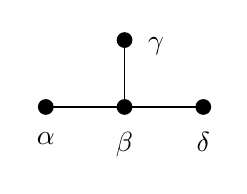
\begin{tikzpicture}
                \draw (1,0) to (2,0);
                \draw (2,0) to (2,0.85);
                \draw (2,0) to (3,0);
                \fill (1,0) circle (1mm);
                \fill (2,0) circle (1mm);
                \fill (2,0.85) circle (1mm);
                \fill (3,0) circle (1mm);
                \draw[below] (1,-0.2) node{$\alpha$};
                \draw[below] (2,-0.2) node{$\beta$};
                \draw[below] (2.4,1) node{$\gamma$};
                \draw[below] (3,-0.2) node{$\delta$};
               \end{tikzpicture}}
\end{figure}

We label $\Psi(G)^{+}$ in the following. The corresponding negative roos are defined accordingly. Note that Roots 1, 2, 3, 4 correspond to $\alpha$, $\gamma$, $\delta$, $\beta$ respectively.
\begin{table}[!h]
\begin{center}
\scalebox{0.7}{
\begin{tabular}{cccccc}
\rootsD{1}{0}{1}{0}{0}&\rootsD{2}{1}{0}{0}{0}&\rootsD{3}{0}{0}{0}{1}&\rootsD{4}{0}{0}{1}{0}&\rootsD{5}{0}{1}{1}{0}&\rootsD{6}{1}{0}{1}{0}\\
\rootsD{7}{0}{0}{1}{1}&\rootsD{8}{1}{1}{1}{0}&\rootsD{9}{0}{1}{1}{1}&\rootsD{10}{1}{0}{1}{1}&\rootsD{11}{1}{1}{1}{1}&\rootsD{12}{1}{1}{2}{1}\\
\end{tabular}
}
\end{center}
\end{table}   
Let
$\lambda:=(\alpha+2\beta+\gamma+\delta)^{\vee}=\alpha^{\vee}+2\beta^{\vee}+\gamma^{\vee}+\delta^{\vee}$. 
Then 
$
P_\lambda=\langle T, U_{\zeta}\mid \zeta\in \Psi(G)^{+}\cup \{-1,-2,-3\} \rangle,
L_\lambda=\langle T, U_{\zeta}\mid \zeta\in \{\pm 1,\pm 2,\pm 3\} \rangle,
R_u(P_\lambda)=\langle U_{\zeta} \mid \zeta \in \Psi(G)^{+}\backslash \{1, 2, 3\} \rangle.
$
Let $a\in k\backslash k^2$. Pick $b\in k^{*}$ with $b^3=1$ and $b\neq 1$. Let $v(\sqrt a):=\epsilon_{4}(\sqrt a)\epsilon_{11}(\sqrt a)\in R_u(P_\lambda)(\overline k)$. Define
\begin{equation*}
H:=v(\sqrt a)\cdot\langle n_\alpha n_\gamma n_\delta, \; (\alpha+\gamma+\delta)^{\vee}(b) \rangle.
\end{equation*}
Here is our first main result in this section.
\begin{prop}\label{firstmain}
$H$ is $k$-defined. Moreover, $H$ is $G$-cr but not $G$-cr over $k$. 
\end{prop}
\begin{proof}
First, we have 
$
(n_\alpha n_\gamma n_\delta) \cdot (\beta) = (n_\alpha n_\gamma n_\delta) \cdot 4 = 11, \;
(n_\alpha n_\gamma n_\delta) \cdot 11 = 4.
$
Using this and the commutation relations~\cite[Lem.~32.5 and Prop.~33.3]{Humphreys-book1}, we obtain
\begin{equation*}
v(\sqrt a)\cdot (n_{\alpha} n_\gamma n_\delta)=(n_\alpha n_\gamma n_\delta) \epsilon_{12}(a).
\end{equation*}
Since $\langle 4, (\alpha+\gamma+\delta)^{\vee}\rangle=-3$, $\langle 11, (\alpha+\gamma+\delta)^{\vee}\rangle=3$, and $b^3=1$, $v(\sqrt a)$ commutes with $(\alpha+\gamma+\delta)^{\vee}(b)$. Now it is clear that $H$ is $k$-defined (since it is generated by $k$-points). 

Now we show that $H$ is $G$-cr. It is sufficient to show that $H':=v(\sqrt a)^{-1}\cdot H=\langle n_\alpha n_\gamma n_\delta,\; (\alpha+\gamma+\delta)^{\vee}(b)$ is $G$-cr since it is $G$-conjugate to $H$. Since $H'$ is contained in $L_\lambda$, by Proposition~\ref{G-cr-L-cr} it is enough to show that $H'$ is $L_\lambda$-cr. By inspection, $H'$ is $L_\lambda$-ir (this is easy since $L_\lambda=L_\alpha\times L_\gamma\times L_\delta=A_1\times A_1 \times A_1$). 


Next, we show that $H$ is not $G$-cr over $k$. Suppose the contrary. Clearly $H$ is contained in $P_\lambda$ that is $k$-defined. Then there exists a $k$-defined Levi subgroup of $P_\lambda$ containing $H$. Then by~\cite[Lem.~2.5(\rmnum{3})]{Bate-uniform-TransAMS} there exists $u\in R_u(P_\lambda)(k)$ such that $H$ is contained in $u\cdot L_\lambda$. Thus $n_\alpha n_\gamma n_\delta \epsilon_{12}(a) < u\cdot L_\lambda$. So $u^{-1}\cdot (n_\alpha n_\gamma n_\delta \epsilon_{12}(a)) < L_{\lambda}$. By~\cite[Prop.~8.2.1]{Springer-book}, we set
$
u:=\prod_{\zeta\in \Psi(R_u(P_\lambda))}\epsilon_\zeta(x_\zeta).
$
Using the labelling of the positive roots above, we have $\Psi(R_u(P_\lambda))=\{4,\cdots 12\}$. We compute how $n_\alpha n_\gamma n_\delta$ acts on $\Psi(R_u(P_\lambda))$: 
\begin{equation}\label{perm}
n_\alpha n_\gamma n_\delta = (4\;11) (5\;10) (6\;9) (7\;8) (12). 
\end{equation}
Using this and the commutation relations,
\begin{alignat*}{2}
u^{-1}\cdot (n_\alpha n_\gamma n_\delta \epsilon_{12}(a))
=&n_\alpha n_\gamma n_\delta \epsilon_4(x_4+x_{11})\epsilon_{5}(x_5+x_{10})\epsilon_{6}(x_6+x_9)\epsilon_{7}(x_{7}+x_{8})\\
&\epsilon_{8}(x_7+x_8)\epsilon_{9}(x_6+x_{9})\epsilon_{10}(x_5+x_{10})\epsilon_{11}(x_4+x_{11})\\
&\epsilon_{12}(x_{4}^2+x_{5}^2+x_{6}^2+x_{7}^2 +a).
\end{alignat*}
Thus if $u^{-1}\cdot (n_\alpha\sigma \epsilon_{\alpha+2\beta+\gamma+\delta}(a)) < L_{\lambda}$ we must have
\begin{equation*}
x_4=x_{11},\; x_5=x_{10},\; x_{6}=x_{9},\; x_7=x_8,\; x_{4}^2+ x_{5}^2+x_{6}^2+x_{7}^2 +a=0.
\end{equation*}
The last equation gives $(x_4+x_5+x_6+x_7)^2=a$. This is impossible since $a\notin k^2$. We are done. 
\end{proof}

\begin{rem}\label{D4nonsep}
From the computations above we see that the curve $C(x):=\{\epsilon_{4}(x)\epsilon_{11}(x)\mid x\in \overline k\}$ is not contained in $C_G(H)$, but the corresponding element in $\textup{Lie}(G)$, that is, $e_4+e_{11}$ is contained in $\mathfrak{c}_{\mathfrak{g}}(H)$. Then the argument in the proof of~\cite[Prop.~3.3]{Uchiyama-Separability-JAlgebra} shows that $\textup{Dim}(C_G(H))$ is strictly smaller than $\textup{Dim}(\mathfrak{c}_{\mathfrak{g}}(H))$. So $H$ is non-separable in $G$. 
In fact, combining~\cite[Thm.~1.5]{Bate-cocharacter-Arx} and~\cite[Thm.~9.3]{Bate-cocharacter-Arx} we have that if a $k$-subgroup $H$ of $G$ is separable in $G$ and $H$ is $G$-cr, then it is $G$-cr over $k$. 
\end{rem}

\vspace{5mm}
Now we move on to the second main result in this section. We use the same $k$, $a$, $b$, $G$, and, $\lambda$ as above. Let $v(\sqrt a):=\epsilon_{-11}(\sqrt a)\epsilon_{-4}(\sqrt a)$. Let
\begin{equation*}
K:=v(\sqrt a)\cdot \langle n_{\alpha} n_{\gamma} n_{\delta},\; (\alpha+\gamma+\delta)^{\vee}(b)\rangle=\langle n_\alpha n_\gamma n_\delta \epsilon_{-12}(a), \;  (\alpha+\gamma+\delta)^{\vee}(b)\rangle. 
\end{equation*}
Define
\begin{equation*}
H:=\langle K, \; \epsilon_{5}(1) \rangle.
\end{equation*}

\begin{prop}\label{secondmain}
$H$ is $k$-defined. Moreover, $H$ is $G$-ir over $k$ but not $G$-cr. 
\end{prop}
\begin{proof}
$H$ is clearly $k$-defined. First, we show that $H$ is $G$-ir over $k$. Note that
\begin{equation*}
v(\sqrt a)^{-1}\cdot H = \langle n_\alpha n_\gamma n_\delta, \; (\alpha+\gamma+\delta)^{\vee}(b),\; \epsilon_{5}(1)\epsilon_{1}(\sqrt a)\rangle.
\end{equation*}
Thus we see that $v(\sqrt a)^{-1}\cdot H$ is contained in $P_\lambda$. So $H$ is contained in $v(\sqrt a)\cdot P_\lambda$. 

\begin{lem}\label{uniquepara}
$v(\sqrt a)\cdot P_\lambda$ is the unique proper parabolic subgroup of $G$ containing $H$.
\end{lem}
\begin{proof}
Suppose that $P_\mu$ is a proper parabolic subgroup of $G$ containing $v(\sqrt a)^{-1}\cdot H$. In the proof of Proposition~\ref{firstmain} we have shown that $M:=\langle n_\alpha n_\gamma n_\delta, (\alpha+\gamma+\delta)^{\vee}(b)\rangle$ is $G$-cr. Then there exists a Levi subgroup $L$ of $P_\mu$ containing $M$ since $M$ is contained in $P_\mu$. Since Levi subgroups of $P_\mu$ are $R_u(P_\mu)$-conjugate by~\cite[Lem.~2.5(\rmnum{3})]{Bate-uniform-TransAMS}, without loss, we set $L:=L_\mu$. Then $M<L_\mu=C_G(\mu(\overline k^*))$, so $\mu(\overline k^*)$ centralizes $M$. Recall that by~\cite[Thm.~13.4.2]{Springer-book}, $C_{R_u(P_\lambda)}(M)^{\circ}\times C_{L_\lambda}(M)^{\circ}\times C_{R_u(P_\lambda^{-})}(M)^{\circ}$ is an open set of $C_G(M)^{\circ}$ where $P_\lambda^{-}$ is the opposite of $P_\lambda$ containing $L_\lambda$.  
\begin{lem}\label{centralizerofM}
$C_G(M)^{\circ}=G_{12}$.
\end{lem}
\begin{proof}
First of all, from Equation~(\ref{perm}) we see that $G_{12}$ is contained in $C_G(n_\alpha n_\gamma n_\delta)$. Since $\langle 12, (\alpha+\gamma+\delta)^{\vee} \rangle=0$, $G_{12}$ is also contained in $C_G((\alpha+\gamma+\delta)^{\vee}(\overline k^*))$. So $G_{12}$ is contained in $C_G(M)$. Set $u:=\prod_{i\in \Psi(R_u(P_\lambda))}\epsilon_{i}(x_i)$ for some $x_i \in \overline k$. Using Equation (\ref{perm}) and the commutation relations, we obtain
\begin{alignat*}{2}
(n_\alpha n_\gamma n_\delta)\cdot u =& \epsilon_{4}(x_{11})\epsilon_{5}(x_{10})\epsilon_{6}(x_9)\epsilon_7(x_{8})\epsilon_8(x_{7})\epsilon_9(x_6)\epsilon_{10}(x_{5})\epsilon_{11}(x_4)\\
&\epsilon_{12}(x_4 x_{11}+x_5 x_{10} +x_6 x_9+ x_7 x_8+ x_{12}). 
\end{alignat*}
So, if $u\in C_{R_u(P_\lambda)}(n_\alpha n_\gamma n_\delta)$ we must have
$x_4=x_{11}, \; x_5=x_{10},\; x_{6}=x_{9},\; x_7=x_8$, and $x_4 x_{11}+x_5 x_{10} +x_6 x_9+ x_7 x_8=0$. But $\langle \zeta, (\alpha+\gamma+\delta)^{\vee}\rangle=-1$ for $\zeta=\{5, 6, 7\}$, so $x_5=x_6=x_7=0$ for $u\in C_{R_u(P_\lambda)}(M)$. Then 
\begin{equation*}
(n_\alpha n_\gamma n_\delta)\cdot u = \epsilon_4(x_4)\epsilon_{11}(x_4)\epsilon_{12}(x_4^2+x_{12}).
\end{equation*}
So we must have $x_4^2=0$ if $u\in C_{R_u(P_\lambda)}(M)$. Thus we conclude that $C_{R_u(P_\lambda)}(M)=U_{12}$. Similarly, we can show that $C_{R_u(P_{\lambda}^{-})}(M)=U_{-12}$. A direct computation shows that $C_{L_\lambda}(M) < T$ and $C_T(n_\alpha n_\gamma n_\delta)=(\alpha+2\beta+\gamma+\delta)^{\vee}(\overline k^*)<G_{12}$. We are done.
\end{proof}
Since $\mu(\overline k^*)$ centralizes $M$, Lemma~\ref{centralizerofM} yields $\mu(\overline k^*)<G_{12}$. Then we can set $\mu:=g\cdot (\alpha+2\beta+\gamma+\delta)^{\vee}$ for some $g\in G_{12}$. By the Bruhat decomposition, $g$ is one of the following forms:
\begin{alignat*}{2}
&(1)\;g=(\alpha+2\beta+\gamma+\delta)^{\vee}(s)\epsilon_{12}(x_1),\\
&(2)\;g=\epsilon_{12}(x_1)n_{12}(\alpha+2\beta+\gamma+\delta)^{\vee}(s)\epsilon_{12}(x_2)\\
&\textup{for some } x_1, x_2\in \overline k, s\in \overline k^*.
\end{alignat*}
We rule out the second case. Suppose $g$ is of the second form. Note that $\epsilon_{5}(1)\epsilon_{1}(\sqrt a)\in v(\sqrt a)^{-1}\cdot H< P_\mu$. 
But $P_\mu=P_{g\cdot (\alpha+2\beta+\gamma+\delta)^{\vee}}=g\cdot P_{(\alpha+2\beta+\gamma+\delta)^{\vee}}$. So it is enough to show that $g^{-1}\cdot (\epsilon_{5}(1)\epsilon_{1}(\sqrt a))\notin P_{(\alpha+2\beta+\gamma+\delta)^{\vee}}$. Since $U_{12}$ and $(\alpha+2\beta+\gamma+\delta)(\overline k^*)$ are contained in $P_{(\alpha+2\beta+\gamma+\delta)^{\vee}}$ we can assume $g=n_{12}$. We have
\begin{equation*}
n_{12}=n_\alpha n_\beta n_\alpha n_\gamma n_\beta n_\alpha n_\delta n_\beta n_\alpha n_\gamma n_\beta n_\delta \textup{ (the longest element in the Weyl group of $D_4$)}.
\end{equation*}
Using this, we can compute how $n_{12}$ acts on each root subgroup of $G$. In particular $n_{12}^{-1}\cdot U_{5}=U_{-5}$ and $n_{12}^{-1}\cdot U_{1}= U_{-1}$. Thus
\begin{alignat*}{2}
n_{12}^{-1}\cdot (\epsilon_{5}(1)\epsilon_{1}(\sqrt a)) &= \epsilon_{-5}(1)\epsilon_{-1}(\sqrt a)\notin P_{(\alpha+2\beta+\gamma+\delta)^{\vee}}.
\end{alignat*}
So $g$ must be of the first form. Then $g\in P_\lambda$. Thus $P_\mu=P_{g\cdot \lambda}=g\cdot P_\lambda=P_\lambda$. We are done.
\end{proof}

\begin{lem}\label{nonkdefined}
$v(\sqrt a)\cdot P_\lambda$ is not $k$-defined.
\end{lem}
\begin{proof}
Suppose the contrary. Since $P_\lambda$ is $k$-defined, $v(\sqrt a)\cdot P_\lambda$ is $G(k)$-conjugate to $P_\lambda$ by~\cite[Thm.~20.9]{Borel-AG-book}. Thus we can put $P_\lambda=g v(\sqrt a)\cdot P_\lambda$ for some $g\in G(k)$. So $g v(\sqrt a)\in P_\lambda$ since parabolic subgroups are self-normalizing. Then $g=pv(\sqrt a)^{-1}$ for some $p\in P_\lambda$. Thus $g$ is a $k$-point of $P_\lambda R_u(P_\lambda^{-})$. Then by the rational version of the Bruhat decomposition~\cite[Thm.~21.15]{Borel-AG-book}, there exists a unique $p'\in P_\lambda(k)$ and a unique $u'\in R_u(P_\lambda^{-})(k)$ such that $g=p' u'$. This is a contradiction since $v(\sqrt a)\notin R_u(P_\lambda^{-})(k)$. 
\end{proof} 
Now Lemmas~\ref{uniquepara},~\ref{nonkdefined} show that $H$ is $G$-ir over $k$. 

\begin{lem}\label{nonG-cr}
$H$ is not $G$-cr. 
\end{lem}
\begin{proof}
We had $C_G(M)^{\circ}=G_{12}$. Then $C_G(v(\sqrt a)^{-1}\cdot H)^{\circ}<G_{12}$ since $M<v(\sqrt a)^{-1}\cdot H$. Using the commutation relations, we see that $U_{12}< C_G(v(\sqrt a)^{-1}\cdot H)$. Note that $v(\sqrt a)^{-1}\cdot H$ contains $h:=\epsilon_{5}(1)\epsilon_{1}(\sqrt a)$ that does not commute with any non-trivial element of $U_{-12}$. Also, since $\langle 5, \lambda\rangle = 4$,  $h$ does not commute with any non-trivial element of $(\alpha+2\beta+\gamma+\delta)^{\vee}(\overline k^*)$.
Thus we conclude that $C_G(v(\sqrt a)^{-1}\cdot H)^{\circ}=U_{12}$. So $C_G(H)^{\circ}=v(\sqrt a)\cdot U_{12}$ which is unipotent. Then by the classical result of Borel-Tits~\cite[Prop.~3.1]{Borel-Tits-unipotent-invent}, we see that $C_G(H)^{\circ}$ is not $G$-cr.
Since $C_G(H)^{\circ}$ is a normal subgroup of $C_G(H)$, by~\cite[Ex.~5.20]{Bate-uniform-TransAMS}, $C_G(H)$ is not $G$-cr. Then by~\cite[Cor.~3.17]{Bate-geometric-Inventione}, $H$ is not $G$-cr. 
\end{proof}
\end{proof}



  
\section{Tits' center conjecture}
In~\cite{Tits-colloq}, Tits conjectured the following:
\begin{con}\label{centerconjecture}
Let $X$ be a spherical building. Let $Y$ be a convex contractible simplicial subcomplex of $X$. If $H$ is an automorphism group of $X$ stabilizing $Y$, then there exists a simplex of $Y$ fixed by $H$.   
\end{con}
This so-called center conjecture of Tits was proved by case-by-case analyses by Tits, M\"{u}hlherr, Leeb, and Ramos-Cuevas~\cite{Leeb-Ramos-TCC-GFA},~\cite{Muhlherr-Tits-TCC-JAlgebra},~\cite{Ramos-centerconj-Geo}. Recently uniform proof was given in~\cite{Weiss-center-Fourier}. In relation to the theory of complete reducibility, Serre showed~\cite{Serre-building}:
\begin{prop}\label{SerreContractible}
Let $G$ be a reductive $k$-group. Let $\Delta(G)$ be the building of $G$. If $H$ is not $G$-cr, then the fixed point subcomplex $\Delta(G)^H$ is  convex and contractible. 
\end{prop}
We identify the set of proper $k$-parabolic subgroups of $G$ with $\Delta(G)$ in the usual sense of Tits~\cite{Tits-book}. Note that for a subgroup $H$ of $G$, $N_G(H)(k)$ induces an automorphism group of $\Delta(G)$ stabilizing $\Delta(G)^H$. Thus, combining the center conjecture with Proposition~\ref{SerreContractible} we obtain
\begin{prop}\label{normalizer}
If a subgroup $H$ of $G$ is not $G$-cr over $k$, then there exists a proper $k$-parabolic subgroup of $G$ containing $H$ and $N_G(H)(k)$. 
\end{prop}
Proposition~\ref{normalizer} was an essential tool to prove various theoretical results on complete reducibility over nonperfect $k$ in~\cite{Uchiyama-Nonperfectopenproblem-pre} and~\cite{Uchiyama-Nonperfect-pre}. We have asked the following in~\cite[Rem.~6.5]{Uchiyama-Nonperfectopenproblem-pre}:
\begin{question}\label{centralizerQ}
If $H<G$ is not $G$-cr over $k$, then does there exist a proper $k$-parabolic subgroup of $G$ containing $HC_G(H)$?
\end{question}
The answer is yes if $C_G(H)$ is $k$-defined (or $k$ is perfect). Since in that case the set of $k$ points are dense in $C_G(H)$ (since we assume $k=k_s$) and the result follows from Proposition~\ref{normalizer}. The main result in this section is to present a counterexample to Question~\ref{centralizerQ} when $k$ is nonperfect. 
\begin{thm}\label{centralizerA}
Let $k$ be nonperfect of characteristic $2$. Let $G$ be simple of type $D_4$. Then there exists a non-abelian $k$-subgroup $H$ of $G$ such that $H$ is not $G$-cr over $k$ but $C_G(H)$ is not contained in any proper $k$-parabolic subgroup of $G$. 
\end{thm}
\begin{rem}
Borel-Tits~\cite[Rem.~2.8]{Borel-Tits-unipotent-invent} mentioned that if $k$ is nonperfect of characteristic $2$ and $[k:k^2]>2$, there exists a $k$-plongeable unipotent element $u$ in $G$ of type $D_4$ such that $C_G(u)$ is not contained in any proper $k$-parabolic subgroup of $G$ (with no proof). Note that such $u$ generates a (cyclic) subgroup of $G$ that is not $G$-cr over $k$. (Recall that a unipotent element is called $k$-plongeable if it can be embedded in the unipotent radical of a proper $k$-parabolic subgroup of $G$~\cite{Borel-Tits-unipotent-invent}.) Theorem~\ref{centralizerA} is a nonabelian version of Borel-Tits' result. Also the assumption $[k:k^2]>2$ is not necessary here. 
\end{rem}
\begin{proof}
We keep the same notation from the previous section. Set $n:=n_\alpha n_\gamma n_\delta$,  $t:=(\alpha+\gamma+\delta)^{\vee}(b)$, and $v(\sqrt a):=\epsilon_4(\sqrt a)\epsilon_{11}(\sqrt a)$. Let $H:=\langle n_\alpha n_\gamma n_\delta \epsilon_{12}(a), (\alpha+\gamma+\delta)^{\vee}(b) \rangle$.  Then $H$ is not $G$-cr over $k$. 
We have $H':=v(\sqrt a)^{-1}\cdot H = \langle n, t \rangle$. It is clear that $C_G(H')>G_{12}$. Thus $\langle n, t, G_{12} \rangle < H'C_G(H')$. By running a similar argument as in the proof of Lemma~\ref{uniquepara} in the previous section, we find that the only proper parabolic subgroup of $G$ containing $\langle n, t, U_{12} \rangle$ is $P_{(\alpha+2\beta+\gamma+\delta)^{\vee}}$ (since $n_{12}\cdot 12 = -12$). Clearly $P_{(\alpha+2\beta+\gamma+\delta)^{\vee}}$ does not contain $G_{12}$. Therefore there is no proper parabolic subgroup of $G$ containing $H'C_G(H')$. Thus there is no proper parabolic subgroup of $G$ containing $HC_G(H)$. 
\end{proof}


\section{G-cr vs $M$-cr (Proof of Theorem~\ref{G-cr-M-cr})}
From this section we assume $k$ is algebraically closed. Let $G$ be as in the hypothesis. Let $a, b\in k^{*}$ with $b^3=1$ and $b\neq 1$. Let $H':=\langle n_\alpha n_\gamma n_\delta, (\alpha+\gamma+\delta)^{\vee}(b) \rangle$. Let $v(a):=\epsilon_4(a)\epsilon_{11}(a)$. Define
\begin{equation*}
H:=v(a)\cdot H' = \langle n_\alpha n_\gamma n_\delta \epsilon_{12}(a^2), (\alpha+\gamma+\delta)^{\vee}(b)\rangle.  
\end{equation*}
Then $H$ is $G$-cr (by the same argument as in the previous section). Now let $M:=\langle G_{\alpha}, G_{\gamma}, G_{\delta}, G_{12}\rangle\cong A_1 A_1 A_1 A_1$. 
\begin{prop}
$H$ is not $M$-cr. 
\end{prop}
\begin{proof}
Let $\lambda:=(\alpha+2\beta+\gamma+\delta)^{\vee}$. Then $H<P_\lambda(M)=\langle T, G_{\alpha}, G_{\gamma}, G_{\delta}, U_{12}\rangle$. Let $c_\lambda: P_\lambda\rightarrow L_\lambda$ be the natural projection. Let $v:=(n_\alpha n_\gamma n_\delta \epsilon_{12}(a^2), (\alpha+\gamma+\delta)^{\vee}(b))$. We have
\begin{equation*}
c_\lambda(v)=\lim_{a\rightarrow 0}\lambda(a)\cdot (n_\alpha n_\gamma n_\delta \epsilon_{12}(a^2), (\alpha+\gamma+\delta)^{\vee}(b))= (n_\alpha n_\gamma n_\delta, (\alpha+\gamma+\delta)^{\vee}(b)).
\end{equation*}
We see that $v$ is not $R_u(P_\lambda(M))$-conjugate to $c_\lambda(v)$ since $R_u(P_\lambda (M))=U_{12}$ centralizes $n_\alpha n_\gamma n_\delta$. By Proposition~\ref{unipotentconjugate}, this shows that $H$ is not $M$-cr. 
\end{proof}
  



\section{K\"ulshammer's question (Proof of Theorem~\ref{thmKul})}
Let $d\geq 5$ be odd. Let $D_{2d}$ be the dihedral group of order $2d$. Let 
\begin{equation*}
\Gamma:=D_{2d}\times C_2 =\langle r, s, z\mid r^d=s^2=z^2=1, srs^{-1}=r^{-1}, [r,z]=[s,z]=1\rangle.
\end{equation*}
Let $\Gamma_2:=\langle s, z\rangle$ (a Sylow $2$-subgroup of $\Gamma$). Let $G$ be as in the hypothesis. Choose $a, b\in k^{*}$ with $b^d=1$ and $b\neq 1$. Let $n:=n_\alpha n_\gamma n_\delta$ and $t:=(\alpha+\gamma+\delta)^{\vee}(b)$. For each $a\in k$ define $\rho_a\in \textup{Hom}(\gamma, G)$ by
\begin{equation*}
\rho_a(r)=t, \; \rho_a(s)=n \epsilon_{12}(a), \; \rho_a(z)=\epsilon_{12}(1). 
\end{equation*}
An easy computation shows that this is well-defined. 
Let $u(\sqrt a)=\epsilon_{4}(\sqrt a)\epsilon_{11}(\sqrt a)$. Then $u(\sqrt a)\cdot n = n\epsilon_{12}(a)$ and $u(\sqrt a)\cdot \epsilon_{12}(1) = \epsilon_{12}(1)$. Thus $u(\sqrt a)\cdot (\rho_0\mid_{\Gamma_2})=\rho_a\mid_{\Gamma_2}$. So $\rho_a\mid_{\Gamma_2}$ are pairwise conjugate. 

Now suppose that $\rho_a$ is conjugate to $\rho_b$. Then there exists $g\in G$ such that $g\cdot \rho_a=\rho_b$. Since $\rho_a(r)=t$, we must have $g\in C_G(t)=TG_{12}$. So let $g=hm$ for some $h\in T$ and $m\in G_{12}$. Then we have
\begin{alignat*}{2}
hnh^{-1}(hm\epsilon_{12}(a)m^{-1}h^{-1})&= hnm\epsilon_{12}(a)m^{-1}h^{-1}\\
                                                                 &= hmn\epsilon_{12}(a)m^{-1}h^{-1}\\
                                                                 &= g\cdot \rho_{a}(s)\\
                                                                 &= \rho_b(s)\\
                                                                 &= n\epsilon_{12}(b).
\end{alignat*}
Note that $hnh^{-1}\in G_\alpha G_\gamma G_\delta$ and $hm\epsilon_{12}(a)m^{-1}h^{-1}\in G_{12}$. Since $[G_\alpha G_\gamma G_\delta, G_{12}]=1$, we have $G_\alpha G_\gamma G_\delta \cap G_{12}=1$. This implies $hnh^{-1}=n$. Now an easy computation shows $h\in G_{12}$. Thus $g=hm\in G_{12}$. Since $G_{12}$ is a simple group of type $A_1$, $(n\epsilon_{12}(a), \epsilon_{12}(1))$ cannot be $G_{12}$- conjugate to $(n\epsilon_{12}(b), \epsilon_{12}(1))$ if $a\neq b$. We are done.                                                                 

\section{Conjugacy classes (Proof of Theorem~\ref{conjugacy-counterexample})}

\begin{proof}
Let $G$ be as in the hypothesis. Let $\lambda:=(\alpha+2\beta+\gamma+\delta)^{\vee}$. Then $\Psi(R_u(P_\lambda))=\{4,\cdots, 12\}$. Using the commutation relations we have $Z(R_u(P_\lambda))=U_{12}$. Let $n:=n_\alpha n_\gamma n_\delta$. Pick $b\in k$ with $b^3=1$ and $b\neq 1$. Let $t:=(\alpha+\gamma+\delta)^{\vee}(b)$. Define $K:=\langle n, t, U_{12} \rangle$. 
By the same argument as that in the proof of~\cite[Lem.~5.1]{Uchiyama-Separability-JAlgebra} we obtain $C_{P_\lambda}(K)=C_{R_u(P_\lambda)}(K)$ (since $\langle 12, \lambda\rangle=2$). By a standard result there exists $n\in \mathbb{N}$ such that $Z=\langle z_1,\cdots, z_n \rangle$. Now let $M:=\langle L_\lambda, G_{12} \rangle$. Let ${\bf m}:=(n, t, z_1,\cdots, z_n)$ and set $N:=n+2$. Then by the similar argument to that in the proof of~\cite[Lem.~5.1]{Uchiyama-Separability-JAlgebra} yields that $G\cdot {\bf m}\cap P_\lambda(M)^N$ is an infinite union of $P_\lambda(M)$-conjugacy classes. (The crucial thing here is the existence of a curve that is tangent to $\mathfrak{c}_{\mathfrak{g}}(K)$ but not tangent to $C_G(K)$, in other words $K$ is nonseparable in $G$.) Now let $c_\lambda:P_\lambda\rightarrow L_\lambda$ be the canonical projection. Then $c_\lambda(n, t, z_1, \cdots, z_n)=(n,t)$. Since $K_0:=\langle n, t \rangle$ is $L$-ir as shown in the previous section, by~\cite[Prop.~3.5.2]{Stewart-thesis} we are done. 
\end{proof}


\section{Acknowledgements}

Luca Herranz-Celotti was supported by the Natural Sciences and Engineering Research Council of Canada through the Discovery Grant from professor Jean Rouat, and by CHIST-ERA IGLU. We thank Compute Canada for the clusters used to perform the experiments and NVIDIA for the donation of two GPUs. We thank Wolfgang Maass for the opportunity to visit the Institute of Theoretical Computer Science, Guillaume Bellec, Darjan Salaj and Franz Scherr, for their invaluable insights on learning with surrogate gradients, and Maryam Hosseini, Ahmad El Ferdaoussi and Guillaume Bellec for their feedback on the article.
\bibliography{mybib}

\end{document}